% !TEX root = ../../main.tex

\section{pyGAPS overview}

After a description of adsorption and its application to porous
material characterisation and prediction of mixture
adsorption, the code which was developed to tackle this type 
of processing can be presented.

The software was imagined for use in two types of scenario.
First, as a command line interface, in common data science environments
such as \texttt{IPython} and \texttt{Jupyter}. The typical user working
in these environments is likely to be processing a small batch of
results at a time, and is interested in obtaining the results in
graphical form. For this type of application, the framework should
provide an unobtrusive way of importing the user data, as well as
present an \gls{API} which does not require extensive knowledge of 
processing methods. Finally, a graphing environment is
required which will allow the user to visualise their
dataset and results.

The second envisaged application is related to bulk data processing.
Requirements here shift towards parameter control, scripting and
extensibility. The framework \gls{API} should offer the option to change 
implicit parameters, select calculation limits and return the results
in a numerical form for further processing. This type of application 
is also likely to require storage of isotherms in a database or
under other types of data files.

\subsection{Core structure}

In order to offer a clear structuring of functionality, 
\texttt{pyGAPS} introduces several classes which abstract data and
concepts for facile interaction (\autoref{pyg:fig:pygaps}). The classes are
intuitively named: \texttt{Isotherm}, \texttt{Sample} and \texttt{Adsorbent}.

\begin{figure}[htb]
    \centering
    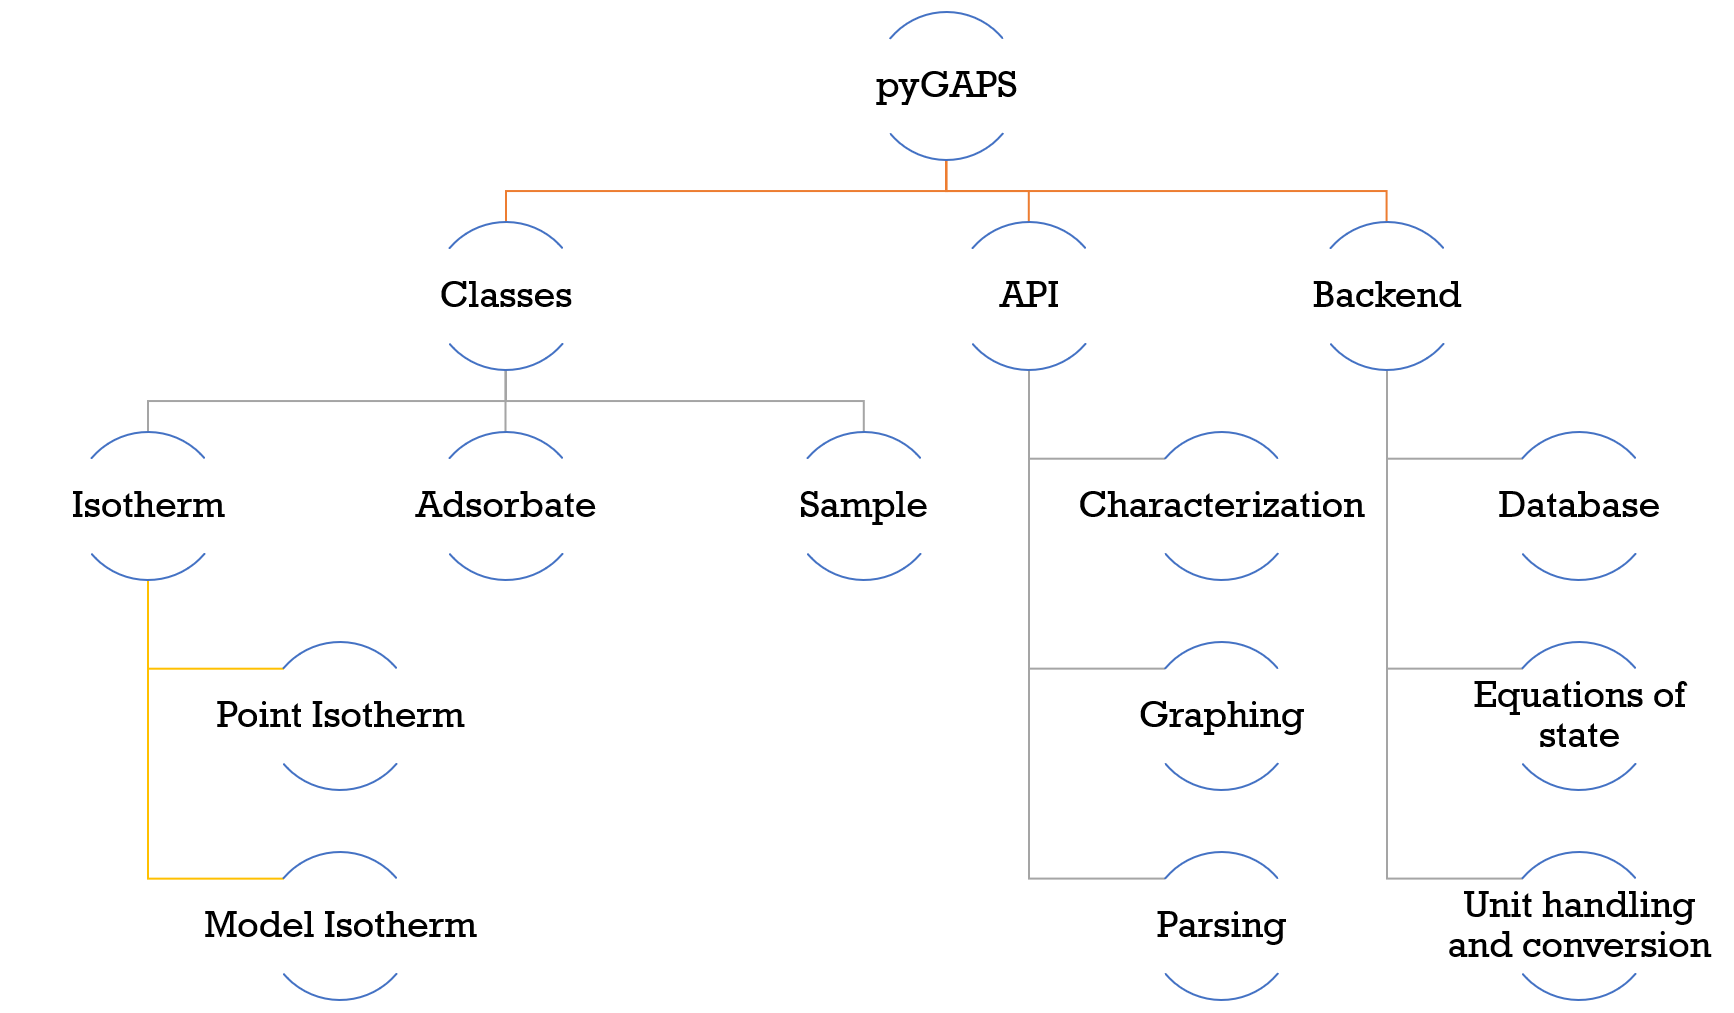
\includegraphics[width=\linewidth]{pygaps}%
	\caption{An overview of the package structure}%
\label{pyg:fig:pygaps}
\end{figure}

\subsubsection{The \texttt{Isotherm} class}

The \texttt{Isotherm} class is a representation of an adsorption 
isotherm i.e.\ a function of the amount adsorbed, or loading, 
versus pressure at a fixed temperature. The class also contains
other information relating to the isotherm, such as the material
name and batch it describes, the adsorbate used and other 
user-defined properties.

This relationship can be defined in two ways:

\begin{itemize}
    \item individual pressure-loading pairs of points which have 
    been recorded as part of a measurement or
    \item a mathematical function describing the relationship 
    between the two properties. 
\end{itemize}

As such, the Isotherm class is used as a parent class for two subclasses: 
the \texttt{PointIsotherm} which contains datapoints and the
\texttt{ModelIsotherm}, containing a model such as Henry, Langmuir etc.
(see \autoref{pyg:models} for the implemented models).
The two classes are interchangeable 
as they share most methods and properties. Once an instance of 
an \texttt{Isotherm} class is created, it can then be used for the 
processing, conversion and graphing capabilities of \texttt{pyGAPS}.

\subsubsection{The \texttt{Sample} class}

The isotherm classes contain the name and batch of the sample 
they are measured on in a string format. The user might want to 
specify other information about the material,
such as the date of synthesis or the material's density,
as well as store this information in the database.
For this case, \texttt{pyGAPS} provides the \texttt{Sample} class.
The framework uses the string values
in the isotherm to connect an \texttt{Isotherm} instance to a 
specific \texttt{Sample}. If sample-related properties are 
needed when processing an isotherms, such as conversion of loading
from a mass basis to a volume basis, this class will be 
checked for the required data.

\subsubsection{The \texttt{Adsorbate} class}

Finally, in order for many of the calculations included in 
\texttt{pyGAPS} to be performed, properties of the adsorbate 
used are needed e.g.\ liquid density, vapour pressure etc.
The \texttt{Adsorbate} class is provided for this purpose,
which is connected to an \texttt{Isotherm} class in an identical manner 
as the \texttt{Sample} class. The physical properties are calculated 
automatically through an equation of state,
either the open source CoolProp library~\cite{bellPurePseudopureFluid2014} 
or the \gls{NIST}-made REFPROP~\cite{lemmonNISTReferenceFluid1989}, if available
on the user's computer. The properties can also be retrieved 
from the internal database or specified by the user.

\subsection{Creation of an Isotherm}

An \texttt{Isotherm} can be created either directly from the command 
line or through an import from a supported format. For direct
creation, the code takes
two kinds of inputs: the data itself, in the form of a 
\texttt{pandas.DataFrame}, and the isotherm parameters describing it.
Only four parameters are strictly required:
the material name, the material batch, the adsorbate used and the 
experimental temperature. Other parameters can be passed as well 
and will be stored in the isotherm class. An example code can 
be seen in \autoref{pyg:lst:isocreation}.

\begin{python}[float=htbp, caption=Creating the \texttt{PointIsotherm},
    label={pyg:lst:isocreation}]
point_isotherm = pygaps.PointIsotherm(

    # First the pandas.DataFrame with the points
    # and the keys to what the columns represent.

    pandas.DataFrame({
        'pressure' : [1, 2, 3, 4, 5, 3, 2],
        'loading' : [1, 2, 3, 4, 5, 3, 2],
        'enthalpy' : [15, 15, 15, 15, 15, 15, 15],
        'xrd_peak_1' : [0, 0, 1, 2, 2, 1, 0],
    }),

    loading_key='loading',          # The loading column
    pressure_key='pressure',        # The pressure column
    other_keys=['enthalpy',
                'xrd_peak_1'],      # The columns containing other data

    # Some of the unit parameters can be 
    # specified if desired.

    pressure_mode='absolute',       # absolute pressure
    pressure_unit='bar',            # with units of bar
    adsorbent_basis='mass',         # adsorbent mass basis
    adsorbent_unit='kg',            # with units of kg
    loading_basis='mass',           # loading mass basis
    loading_unit='g',               # with units of g

    # Finally the isotherm description
    # parameters are passed.

    sample_name='carbon',           # Required
    sample_batch='X1',              # Required
    adsorbate='nitrogen',           # Required
    t_exp=77,                       # Required
    t_act=150,                      # Recognised / named
    user='Username',                # Recognised / named
    DOI='10.000/mydoi',             # Unknown / user specific
}
\end{python}

The \texttt{DataFrame} must contain a column with the pressure
points and one with the corresponding loading points of the 
isotherm. Other columns can also be passed, when
secondary data such as enthalpy of adsorption is present at 
each measurement point. These columns will be saved in the case of
the \texttt{PointIsotherm} class and can be
plotted afterwards. The framework can automatically attempt to 
determine the adsorption and desorption branches, by analysing the
input data. Alternatively, the user can manually specify which
points belong to each branch.

If no unit data is specified in the constructor, the framework will
assume that the isotherm is in units of \si{\milli\mole\per\gram} 
loading as a function of \si{\bar}. Both the units and the basis 
can be specified, as it is explained in a latter section.

Finally, the data is saved in the newly created class or used to
generate parameters for a model such as \gls{BET}, Langmuir, etc.,
in the case of a \texttt{PointIsotherm} and
\texttt{ModelIsotherm} respectively. The creation of
\texttt{Sample} and \texttt{Adsorbate} instances is similar.

Alternatively, the isotherm can be imported from a file containing 
a format that is recognised by \texttt{pyGAPS}. Parsing from 
suitably structured JSON, CSV and Excel files is supported.

Both \texttt{PointIsotherm}s and \texttt{ModelIsotherm} can
be created from an instance of the other, by using the 
available functions. As an example, a \texttt{ModelIsotherm} is automatically
generated from the previous isotherm using the function in
\autoref{lst:model}, which fits all available models and selects
the one with the lowest residuals between the fitted function
and the real data.

\begin{python}[caption={Guessing the best model},label={lst:model}]
model = pygaps.ModelIsotherm.from_pointisotherm(iso, guess_model=True)
\end{python}
\begin{pythonout}
Attempting to model using Henry
Model Henry success, rmse is 7.42
Attempting to model using Jensen-Seaton
Modelling using Jensen-Seaton failed
...............................
Best model fit is Quadratic
\end{pythonout}

\subsection{Units}

When computers work with physical data, units are often a matter 
that introduces confusion. Therefore \texttt{pyGAPS} should
carefully handle units and other physical world concepts such as relative
pressure and mass or volume basis.

The following dimensions can be specified for an Isotherm: 
the measurement \textit{pressure}, the quantity of guest adsorbed
or \textit{loading} and the amount of adsorbent material
the loading is reported on, or \textit{adsorbent}.

Pressure can be reported either in an absolute value, in several 
common units such as \si{\bar}, torr, \si{\pascal}, or as 
\textit{relative pressure}, absolute pressure divided by the 
saturation vapour pressure of the adsorbate at the respective
measurement temperature. Conversions between the two modes are 
automatic and handled internally.

Both the \textit{loading} and \textit{adsorbent} can be reported
in three different bases: a molar basis, a mass basis or a volume
basis. Within each basis different units are recognised and can be
easily converted. The conversions between bases can also
easily performed if the required conversion factors (i.e.\ molar 
mass and density) are available. For \textit{loading}, these 
factors are automatically calculated internally using the 
available equation of state, while for the \textit{adsorbent} 
they should be provided by the user in the respective \texttt{Sample}
 class.

\subsection{Workflow}

Once an isotherm object is created, it will be used for all 
further processing. The class contains methods which can be 
used to inspect the data visually, or retrieve
parts of the isotherm such as the adsorption or desorption branches with
user-chosen limits or units. Singular values of pressure or 
loading can be calculated, either through interpolation in the
case of a \texttt{PointIsotherm} or by evaluation
of the internal model in the \texttt{ModelIsotherm}. For an isotherm with
datapoints, these can also be converted into different units or modes.
A common first step is to display the created isotherm using the 
\inline{.print_info()} function, which displays all information in a
class, as exemplified in \autoref{appx:lst:print_info}.

Characterisation functions take an \texttt{Isotherm} object as their
first parameter. This is the case for the \gls{BET} area, Langmuir area, 
t-plot, \(\alpha_s\) plot, and pore size distribution methods.
These characterisation functions attempt to automate as much
of the process as possible. For example, the \gls{BET} area limits are
automatically calculated using the 
Rouquerol~\cite{rouquerolAdsorptionPowdersPorous2013} method, 
with all the checks implemented into the code. As another example,
the straight line sections of the t-plot are determined automatically
through a calculation of the second derivative of the transformed isotherm.
For detailed control, there are available options for each individual 
method, such as manual \gls{BET} limits, different thickness functions for
the t-plot or Kelvin-based mesoporous pore distribution methods, 
custom parameters for the Horvath-Kawazoe microporous pore
distribution, custom \gls{DFT} or \gls{NLDFT} kernels and more. The results are
returned in a numerical form for further processing, or can be directly
displayed if the \texttt{verbose} parameter is passed.

\subsection{Characterisation using pyGAPS}

\subsubsection{\gls{BET} and Langmuir surface area}

\texttt{pyGAPS} comes with several common methods used to
determine surface area, some with theoretical basis like
the \gls{IUPAC}-recommended \gls{BET} method and some empirical, such
as the t-plot method.

Starting from an isotherm object, it is easy to
calculate the nitrogen \gls{BET} area of a sample of UiO-66(Zr) \gls{MOF}
by using the code in \autoref{pyg:lst:betarea}.
The framework automatically applies the methodology described in
\autoref{pyg:charac:betarea} to find the optimum pressure range. 
The \inline{verbose=True} option prints a short
text with all the calculation variables as well as graphing the
\gls{BET} and Rouquerol plots (\autoref{pyg:fig:betarea}).
The user can override automatic pressure range selection by using the
range parameter (\inline{limits=(0.05, 0.3)}).

\begin{samepage}
	\begin{python}[caption={Calculating a BET area},label={pyg:lst:betarea}]
area_dict = pygaps.area_BET(isotherm, verbose=True)
\end{python}
	\begin{pythonout}
BET surface area: a = 1277 m2/g
Minimum pressure point chosen is 0.005 and maximum is 0.034
The slope of the BET fit: 		s = 76.344
The intercept of the BET fit: 	i = 0.052
BET constant: 					C = 1463
Amount for a monolayer: 		n = 0.01309 mol/g
\end{pythonout}
\end{samepage}

\begin{figure}[!htb]
	\centering

	\begin{subfigure}{0.45\linewidth}
		\parbox[c]{0.1\linewidth}{\caption{}%
			\label{pyg:fig:betarea-plt}}
		\parbox[b]{0.85\linewidth}{%
			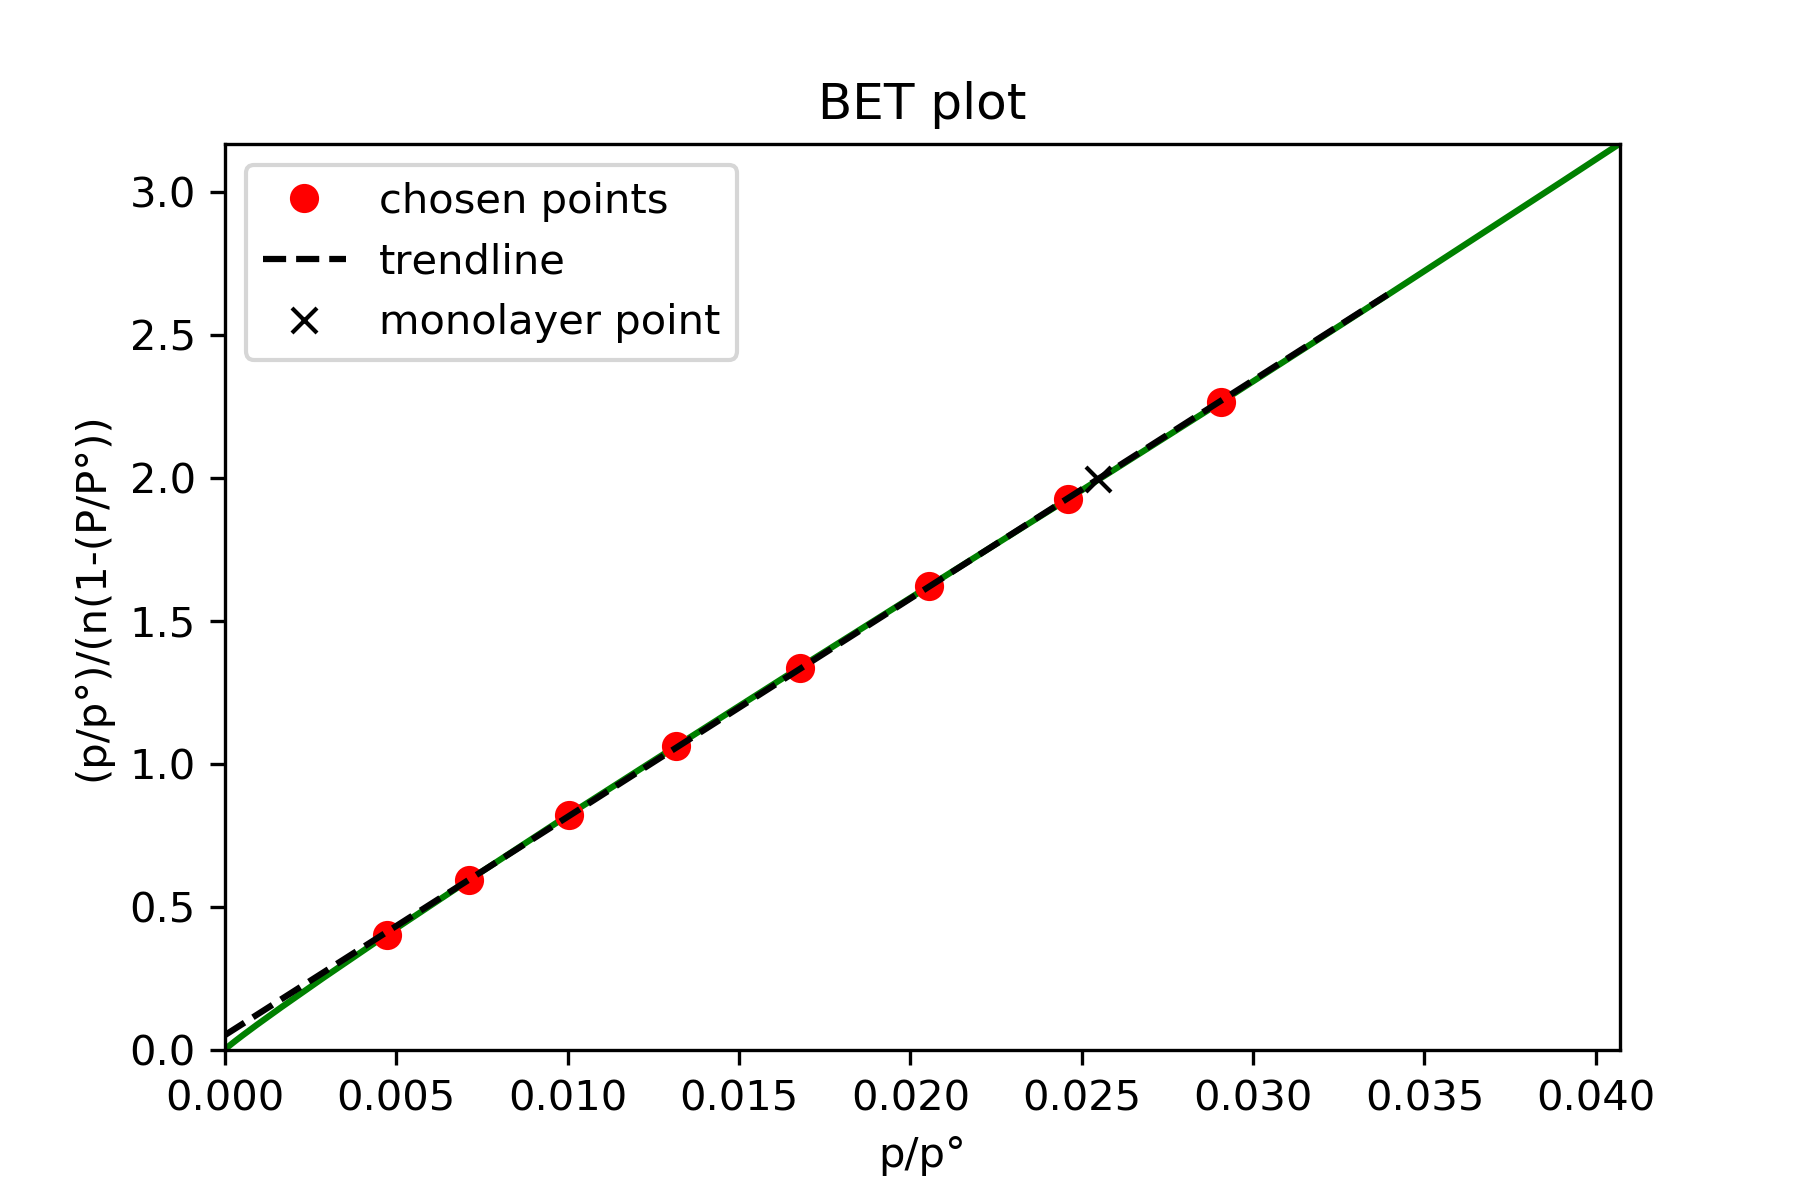
\includegraphics[width=\linewidth]{characterization/bet-plt}}
	\end{subfigure}%
	\begin{subfigure}{0.45\linewidth}
		\parbox[c]{0.1\linewidth}{\caption{}%
			\label{pyg:fig:betarea-roq}}
		\parbox[b]{0.85\linewidth}{%
			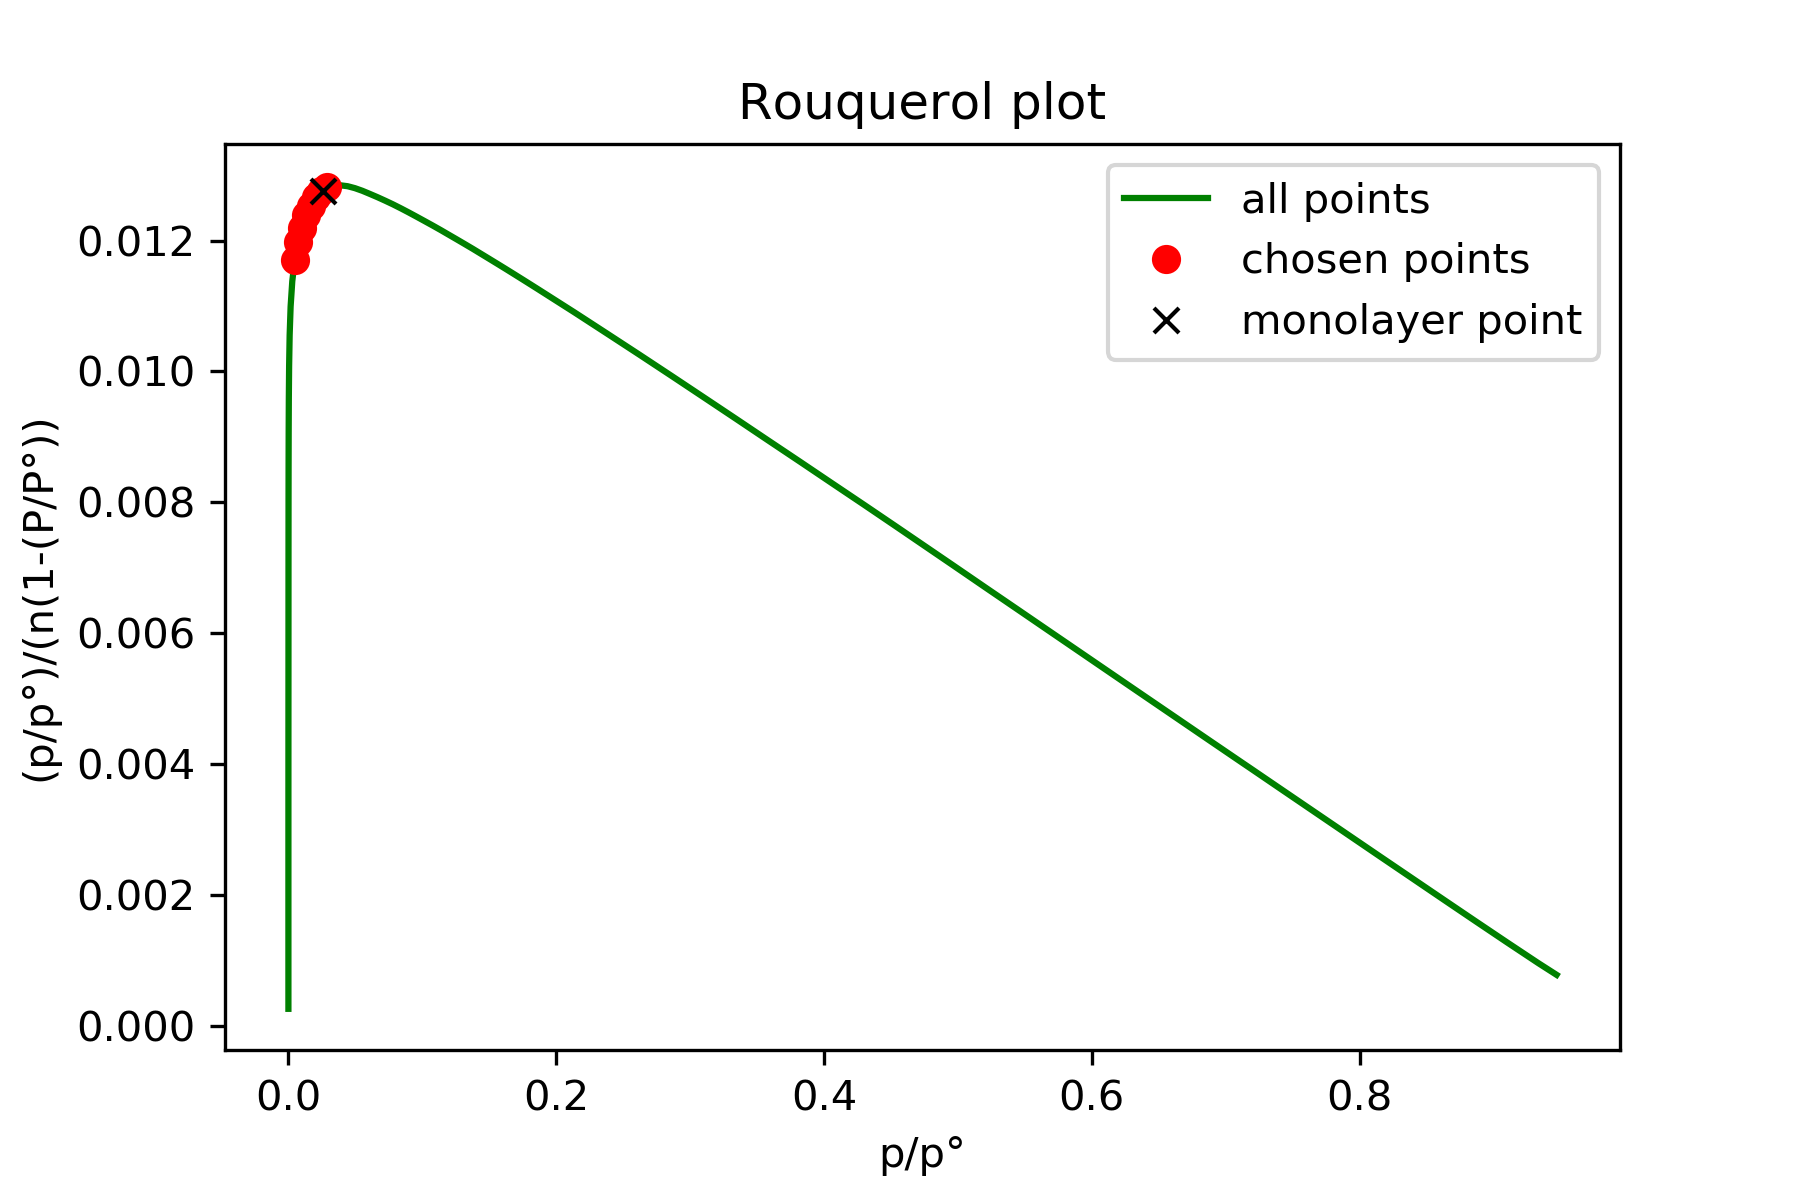
\includegraphics[width=\linewidth]{characterization/bet-roq}}
	\end{subfigure}%

	\caption{Output from the \gls{BET} area function (a) the \gls{BET} plot showing
		the selected points for fitting the equation, as well as the location
		of the statistical monolayer and (b) the Rouquerol plot for this
		calculation.}%
	\label{pyg:fig:betarea}

\end{figure}

Similarly to the \gls{BET} area, the Langmuir area is calculated by using
the code in \autoref{pyg:lst:langmuirarea}. The framework will alert
the user if the correlation is not linear in the selected range.
In this example, the surface area of a nitrogen isotherm measured 
on a MCM-41 sample is calculated.
Here the \inline{verbose=True} option prints a short
text with all the calculation results, as well as generating the
Langmuir plot as seen in \autoref{pyg:fig:langmuirarea-auto}.
If desired the user can override automatic pressure range selection
as seen in the second example in \autoref{pyg:lst:langmuirarea}.

\begin{samepage}
	\begin{python}[caption={Calculating a Langmuir area},label={pyg:lst:langmuirarea}]
area_dict = pygaps.area_langmuir(isotherm, verbose=True)
\end{python}
	\begin{pythonout}
WARINING The correlation is not linear!
\end{pythonout}
	\begin{python}
area_dict = pygaps.area_langmuir(isotherm, 
                                 limits=(0.05, 0.3), 
                                 verbose=True)
\end{python}
	\begin{pythonout}
Langmuir surface area: 	a = 415 m2/g
Minimum pressure point chosen is 0.0 and maximum is 0.194
The slope of the Langmuir line: 		s = 234.968
The intercept of the Langmuir line: 	i = 1.607
The Langmuir constant is:				K = 146
Amount for a monolayer: 				n = 0.00426 mol/g
\end{pythonout}
\end{samepage}

\begin{figure}[!htb]
	\centering

	\begin{subfigure}{0.45\linewidth}
		\parbox[c]{0.1\linewidth}{\caption{}%
			\label{pyg:fig:langmuirarea-auto}}
		\parbox[b]{0.85\linewidth}{%
			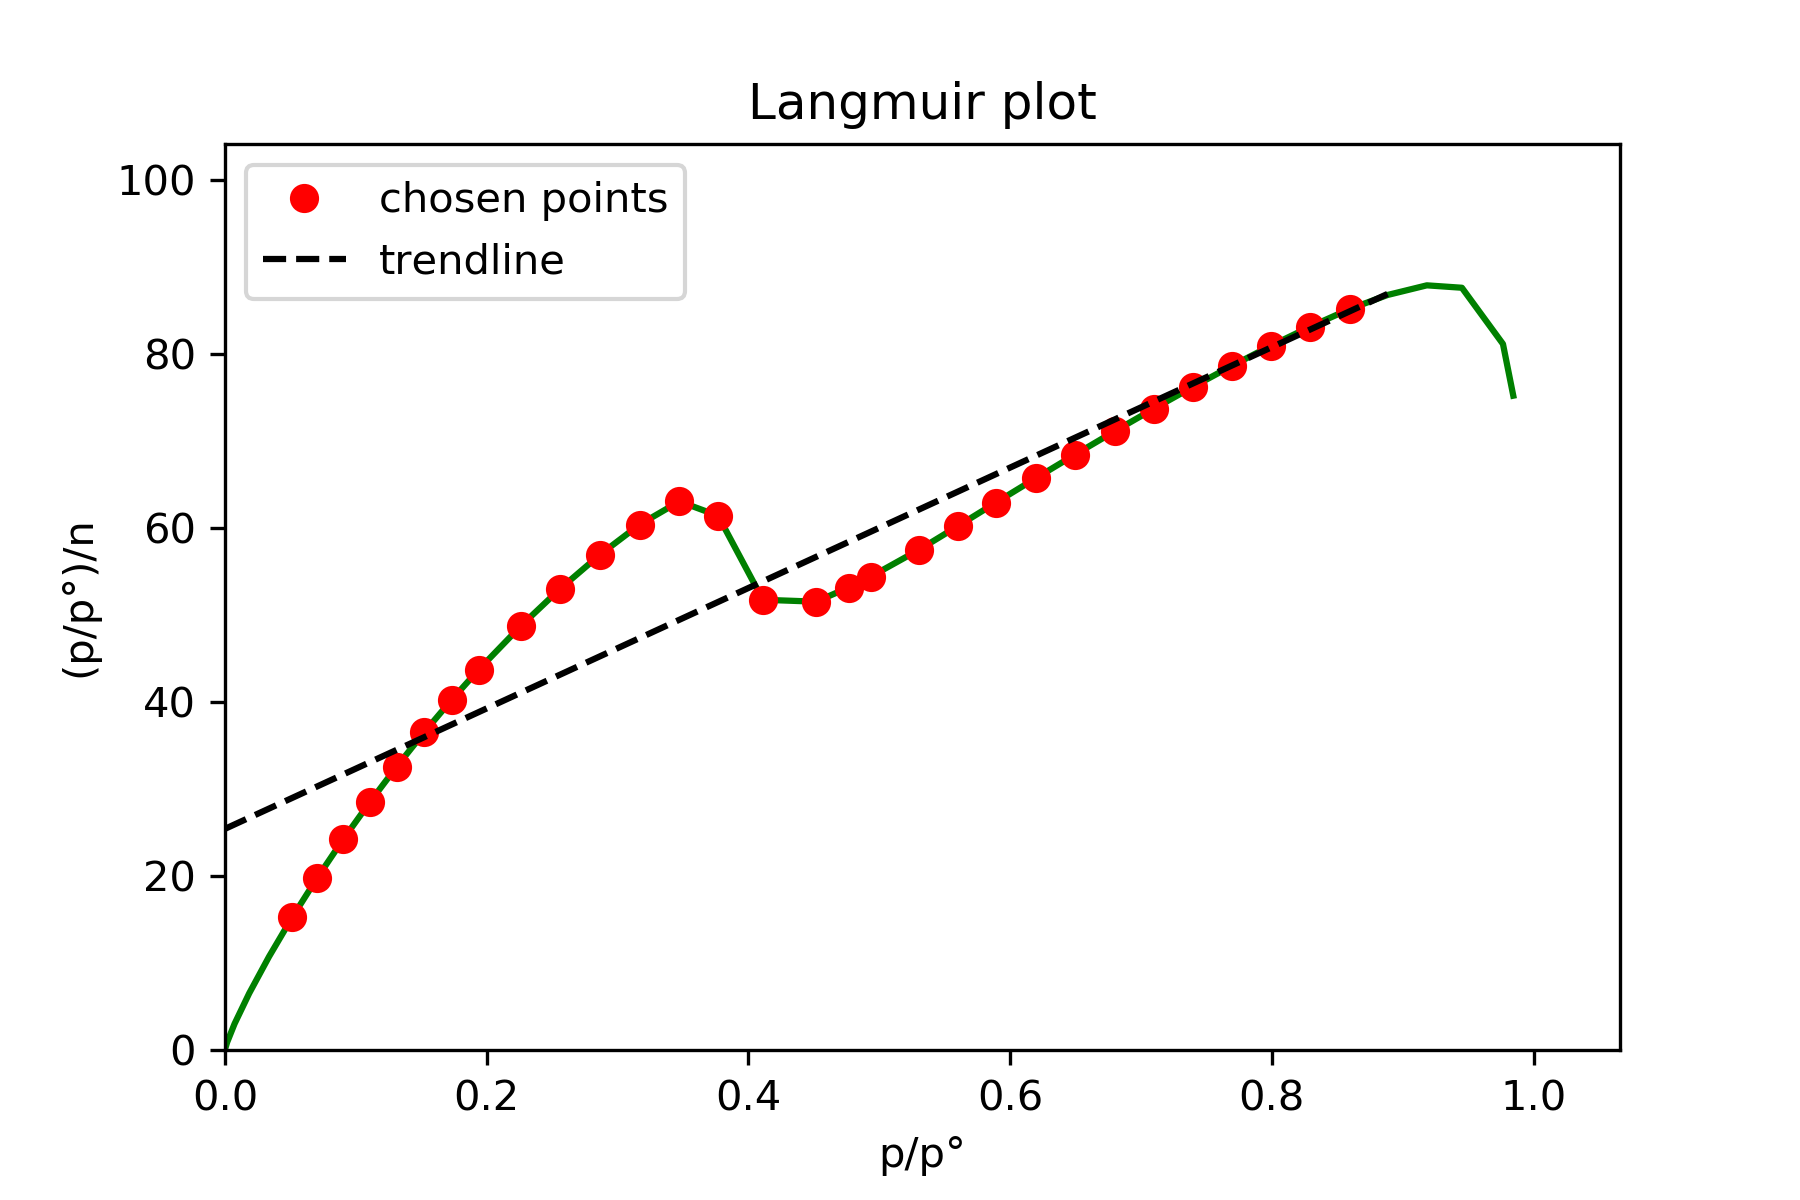
\includegraphics[width=\linewidth]{characterization/langmuir-auto}}
	\end{subfigure}%
	\begin{subfigure}{0.45\linewidth}
		\parbox[c]{0.1\linewidth}{\caption{}%
			\label{pyg:fig:langmuirarea-manual}}
		\parbox[b]{0.85\linewidth}{%
			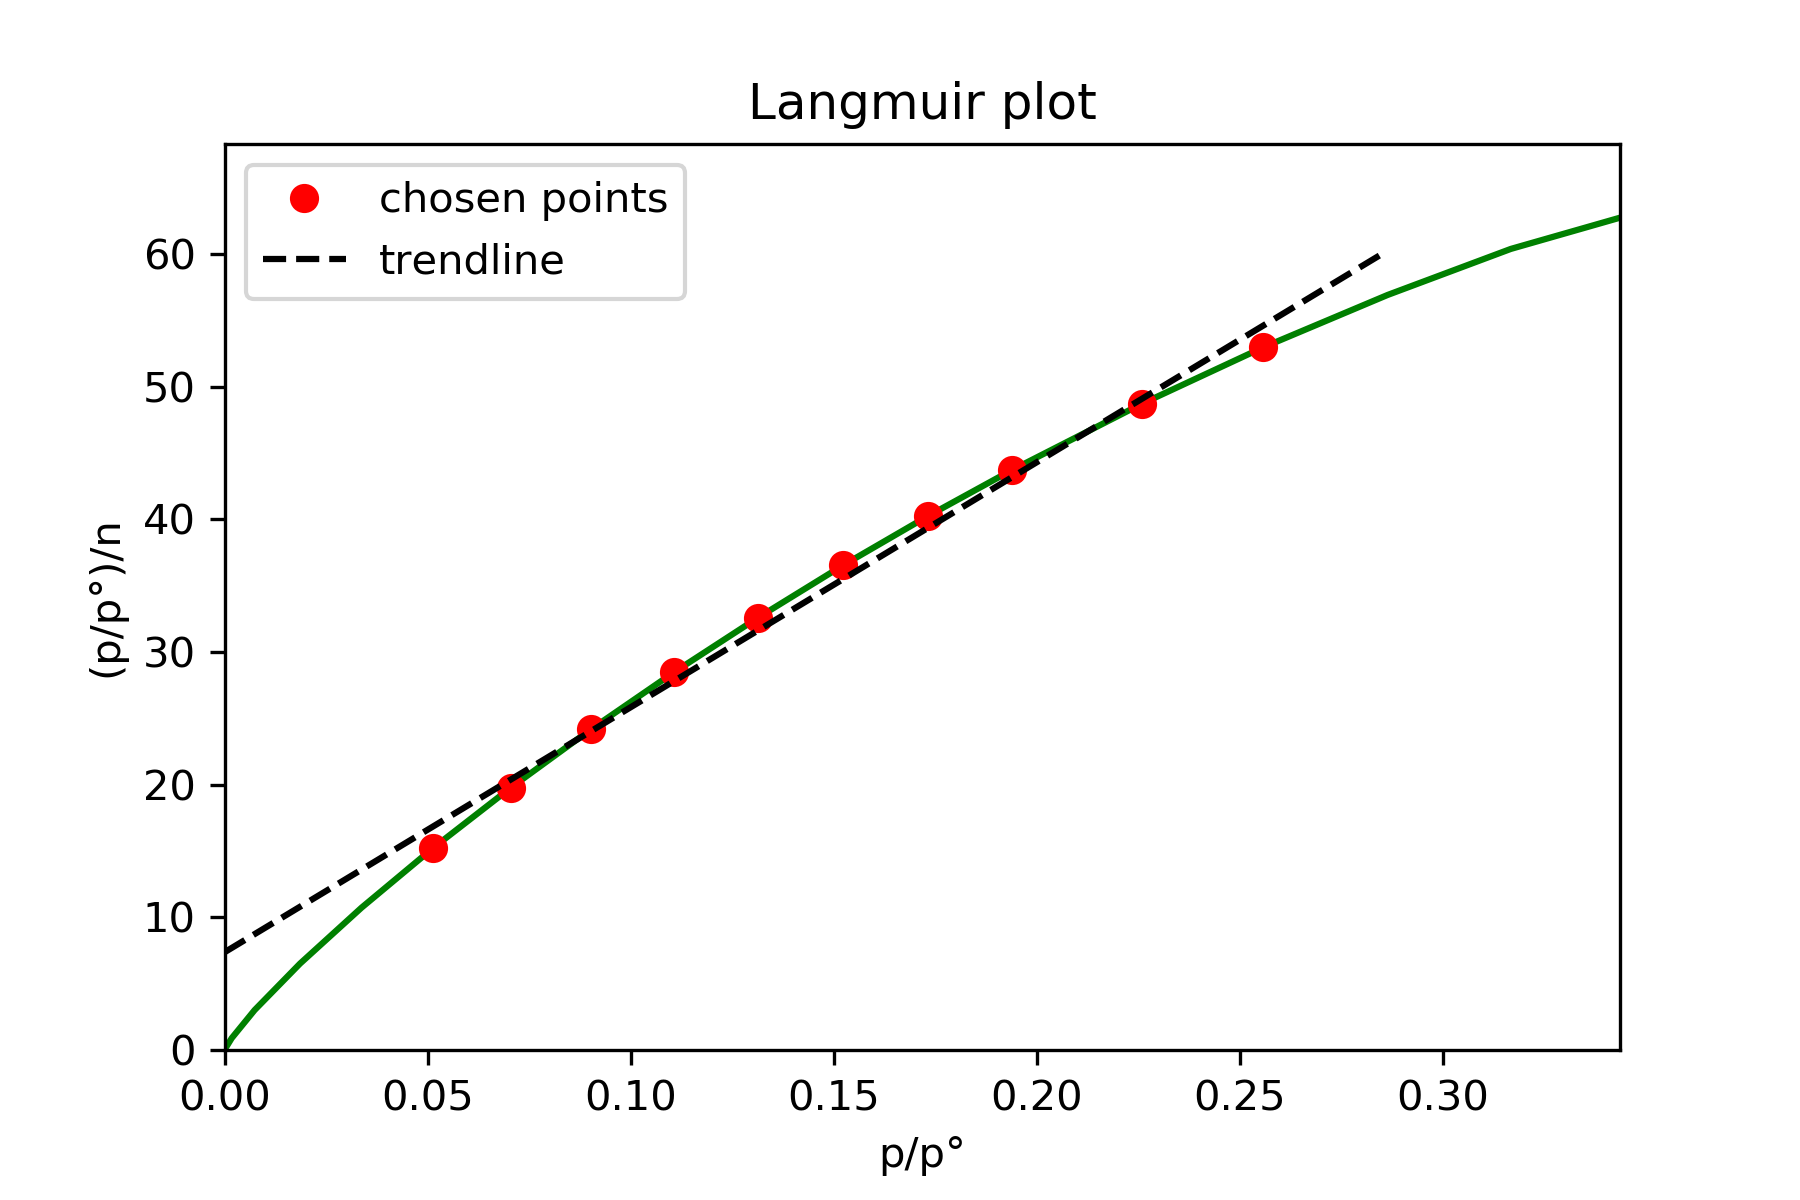
\includegraphics[width=\linewidth]{characterization/langmuir-manual}}
	\end{subfigure}%

	\caption{Output from the Langmuir area function (a) the Langmuir plot
		showing the automatic fitting attempt which generates a warning and (b) a manually
		selected pressure range for the Langmuir plot.}%
	\label{pyg:fig:langmuirarea}

\end{figure}

\subsubsection{The t-plot Method and \(\alpha_s\) Method}

The t-plot method requires a model for the thickness of 
the adsorbed layer, as described in \autoref{pyg:charac:tcurve}.
The two equations presented there have been implemented in \texttt{pyGAPS}.
These t-curves are selected by name as parameters in
the functions that use them. The user can also define their
own t-curve as a function and pass it as a parameter.

When the t-plot function is called without any parameters
except an isotherm, the framework will attempt to find 
plateaus in the data and
automatically fit them with a straight line, returning a dictionary
with the slope, intercept, calculated pore volume and specific area
for each linear region found. 
The same MCM-41 nitrogen isotherm analysed in the previous section is
used in \autoref{pyg:lst:tplot}. The first command will generate the
graph in \autoref{pyg:fig:tplot-auto}. 

\begin{python}[float=htb, caption={Generating a t-plot},%
    label={pyg:lst:tplot}]
# using automatic region detection
pygaps.t_plot(isotherm, verbose=True)

# specifying a manual region
pygaps.t_plot(isotherm, limits=(0.3,0.44), verbose=True)

# using the Halsey thickness curve
pygaps.t_plot(isotherm, thickness_model='Halsey', verbose=True)

# defining a custom t-curve to use in the t-plot
def carbon_model(relative_p):
	return 0.88*(relative_p**2) + 6.45*relative_p + 2.98

pygaps.t_plot(isotherm, thickness_model=carbon_model, verbose=True)
\end{python}

\begin{figure}[!htb]
	\centering

	\begin{subfigure}{0.45\linewidth}
		\parbox[c]{0.1\linewidth}{\caption{}%
			\label{pyg:fig:tplot-auto}}
		\parbox[b]{0.85\linewidth}{%
			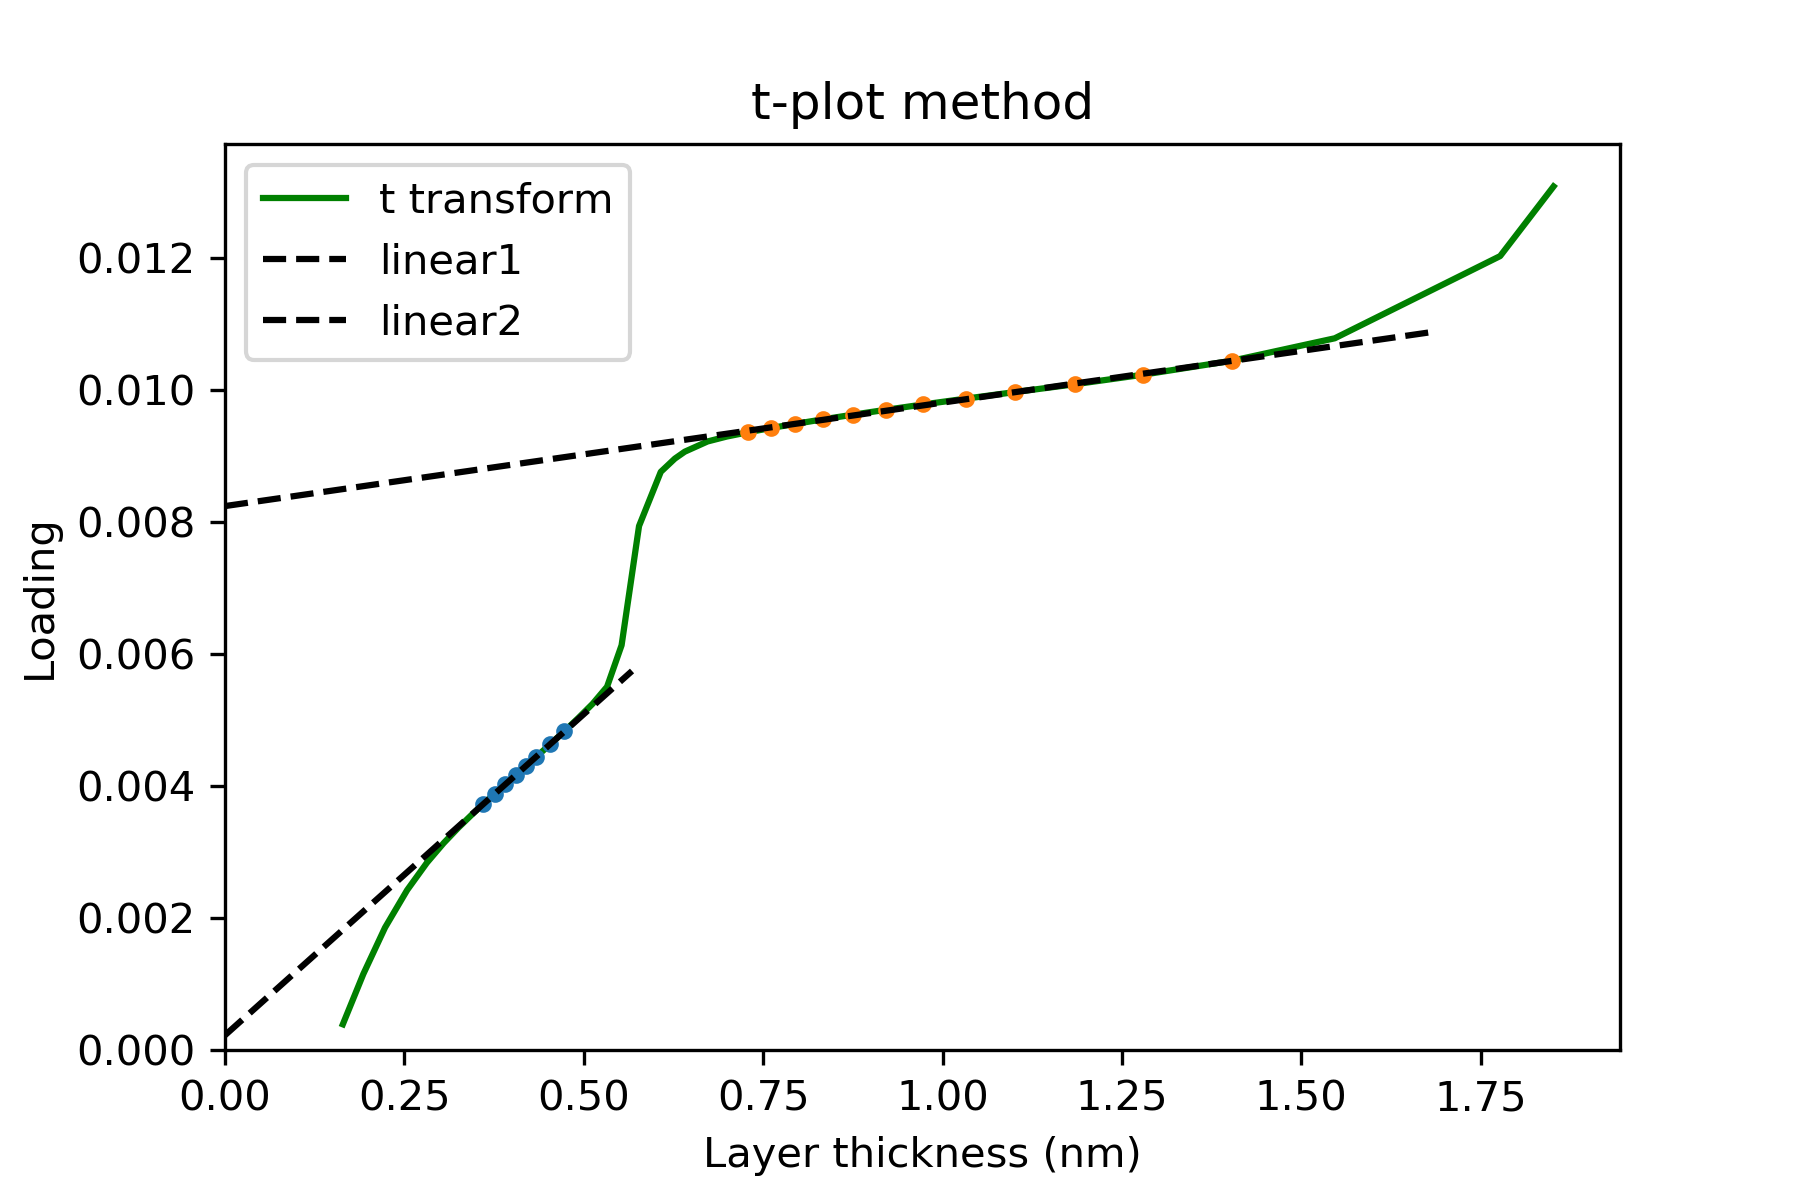
\includegraphics[width=\linewidth]{characterization/tplot-auto}}
	\end{subfigure}%
	\begin{subfigure}{0.45\linewidth}
		\parbox[c]{0.1\linewidth}{\caption{}%
			\label{pyg:fig:tplot-manual}}
		\parbox[b]{0.85\linewidth}{%
			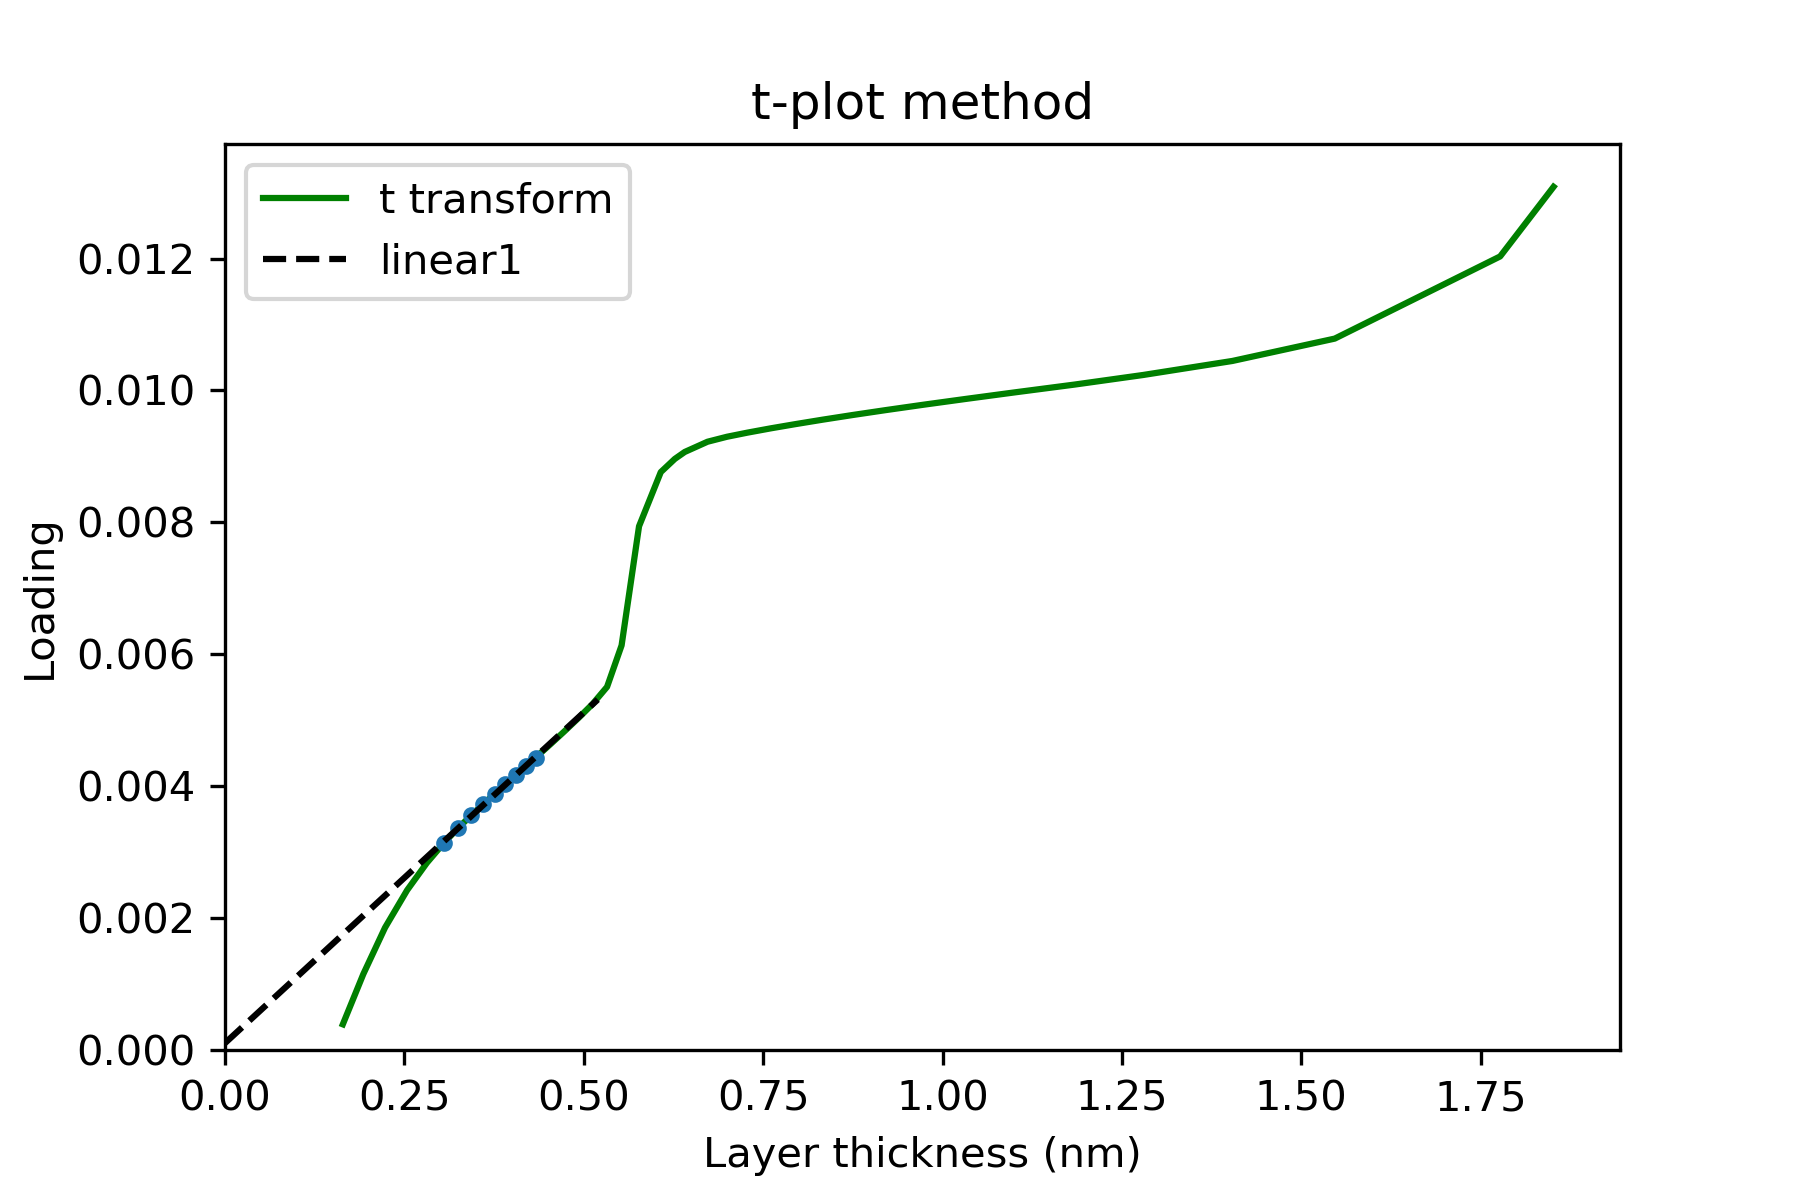
\includegraphics[width=\linewidth]{characterization/tplot-manual}}
	\end{subfigure}%

	\caption{Output from the t-plot method function (a) an automatically
		obtained t-plot with the calculated fit regions and (b) a manually
		selected range for the t-plot.}%
	\label{pyg:fig:tplot}

\end{figure}

The first linear region in \autoref{pyg:fig:tplot-auto} can be attributed
to adsorption on the mesopore surface,
while the second one represents adsorption on the available surface
after mesopore filling. Therefore, the surface area values calculated 
for the first and second region correspond to the area of the mesopores
and the external particle area, respectively. As only one pore filling 
event occurs, the pore volume calculated for the second region gives
us the mesopore volume. We can obtain a more accurate result for the
surface area by fitting the first linear region to a zero intercept
through manual region selection, as shown in the second example in 
\autoref{pyg:lst:tplot}.

Finally, the framework allows for the thickness model to be substituted
with an user-provided function which will be used for the t-plot.
Usage of a carbon black-type thickness curve is presented in the last
example in \autoref{pyg:lst:tplot}.

To generate an \(\alpha_s\)-plot in \texttt{pyGAPS}, both 
an analysis isotherm and a reference isotherm must be supplied 
as shown in \autoref{pyg:lst:alphasplot}, using the same isotherm
as for the t-plot.
In this example, the reference isotherm is measured on non-porous 
silica. The reference material area can be specified by using 
the \inline{reference_area} parameter. If not specified, it 
is automatically calculated by applying the \gls{BET}
method to the reference isotherm.

\begin{python}[caption={Generating an \(\alpha_s\)-plot},label={pyg:lst:alphasplot}]
pygaps.alpha_s(isotherm, 
			   reference_isotherm=isotherm_r,
			   verbose=True)
\end{python}

\begin{figure}[!htb]
	\centering

	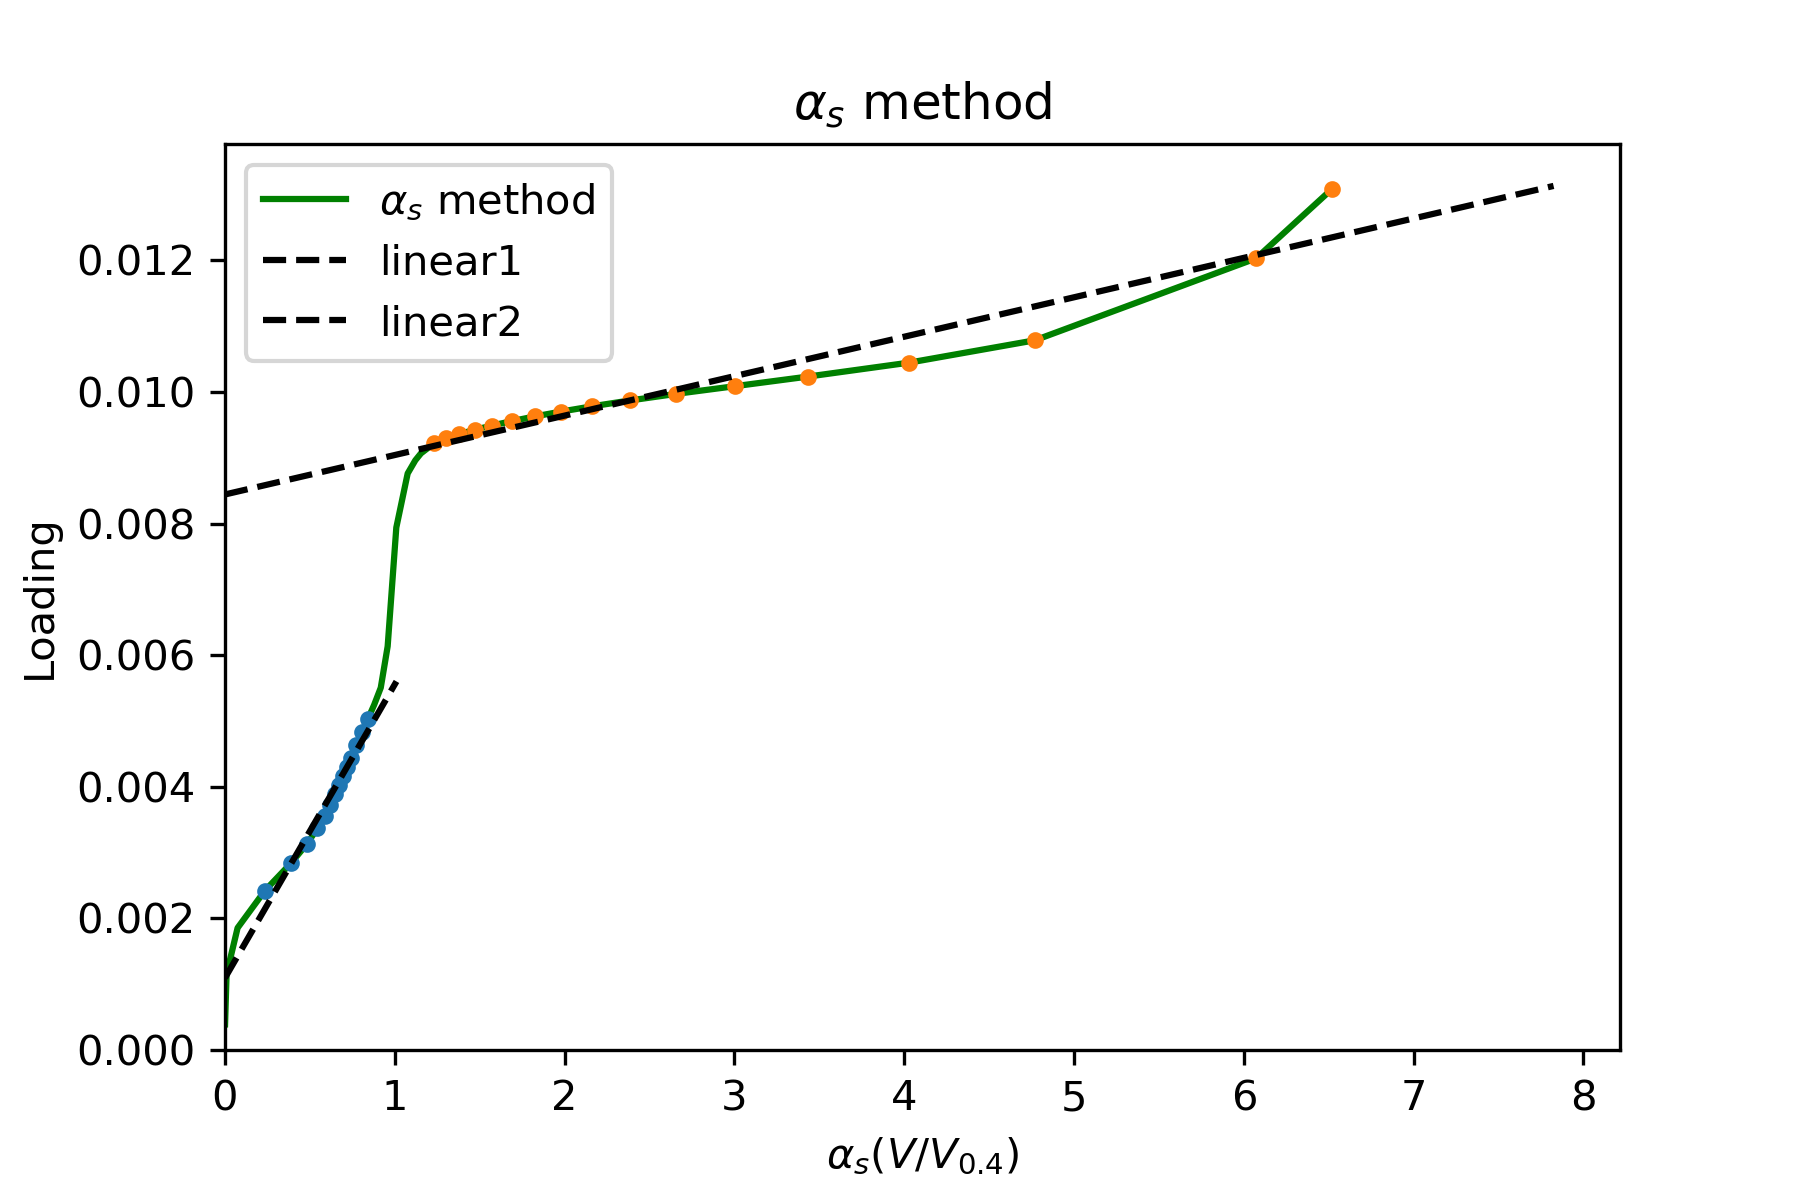
\includegraphics[width=0.45\linewidth]{characterization/alphas-auto}
	\caption{Output from the \(\alpha_s\)-plot function showing two
		automatically fit regions.}%
	\label{pyg:fig:alphasplot}

\end{figure}


\subsubsection{Pore size distribution calculations}

Both mesoporous, microporous and \gls{DFT} fitting routines can be
used to calculate a pore size distribution in \texttt{pyGAPS}. 
While the generation of \gls{DFT} kernels is outside the scope of the
framework, the code able to use user-provided kernels to fit adsorption 
isotherms, and comes with a basic kernel applicable for \ce{N2} 
adsorption at \SI{77}{\kelvin} on carbon slit pores.

The MCM-41 sample is a mesoporous material, which is expected
to have a well-defined pore size in the range of 
\SIrange{2.5}{5}{\nano\metre}. The \gls{BJH} method can be readily
applied on the desorption branch of the measured isotherm, through
the code in \autoref{pyg:lst:bjh}. The Harkins and Jura thickness
function is automatically selected, while the default cylindrical pore 
geometry is used.

\begin{python}[caption={PSD using the BJH method},%
    label={pyg:lst:bjh}]
result_dict = pygaps.mesopore_size_distribution(
    charact_iso,
    psd_model='BJH',
    verbose=True
)
\end{python}

\begin{figure}[!htb]
	\centering
	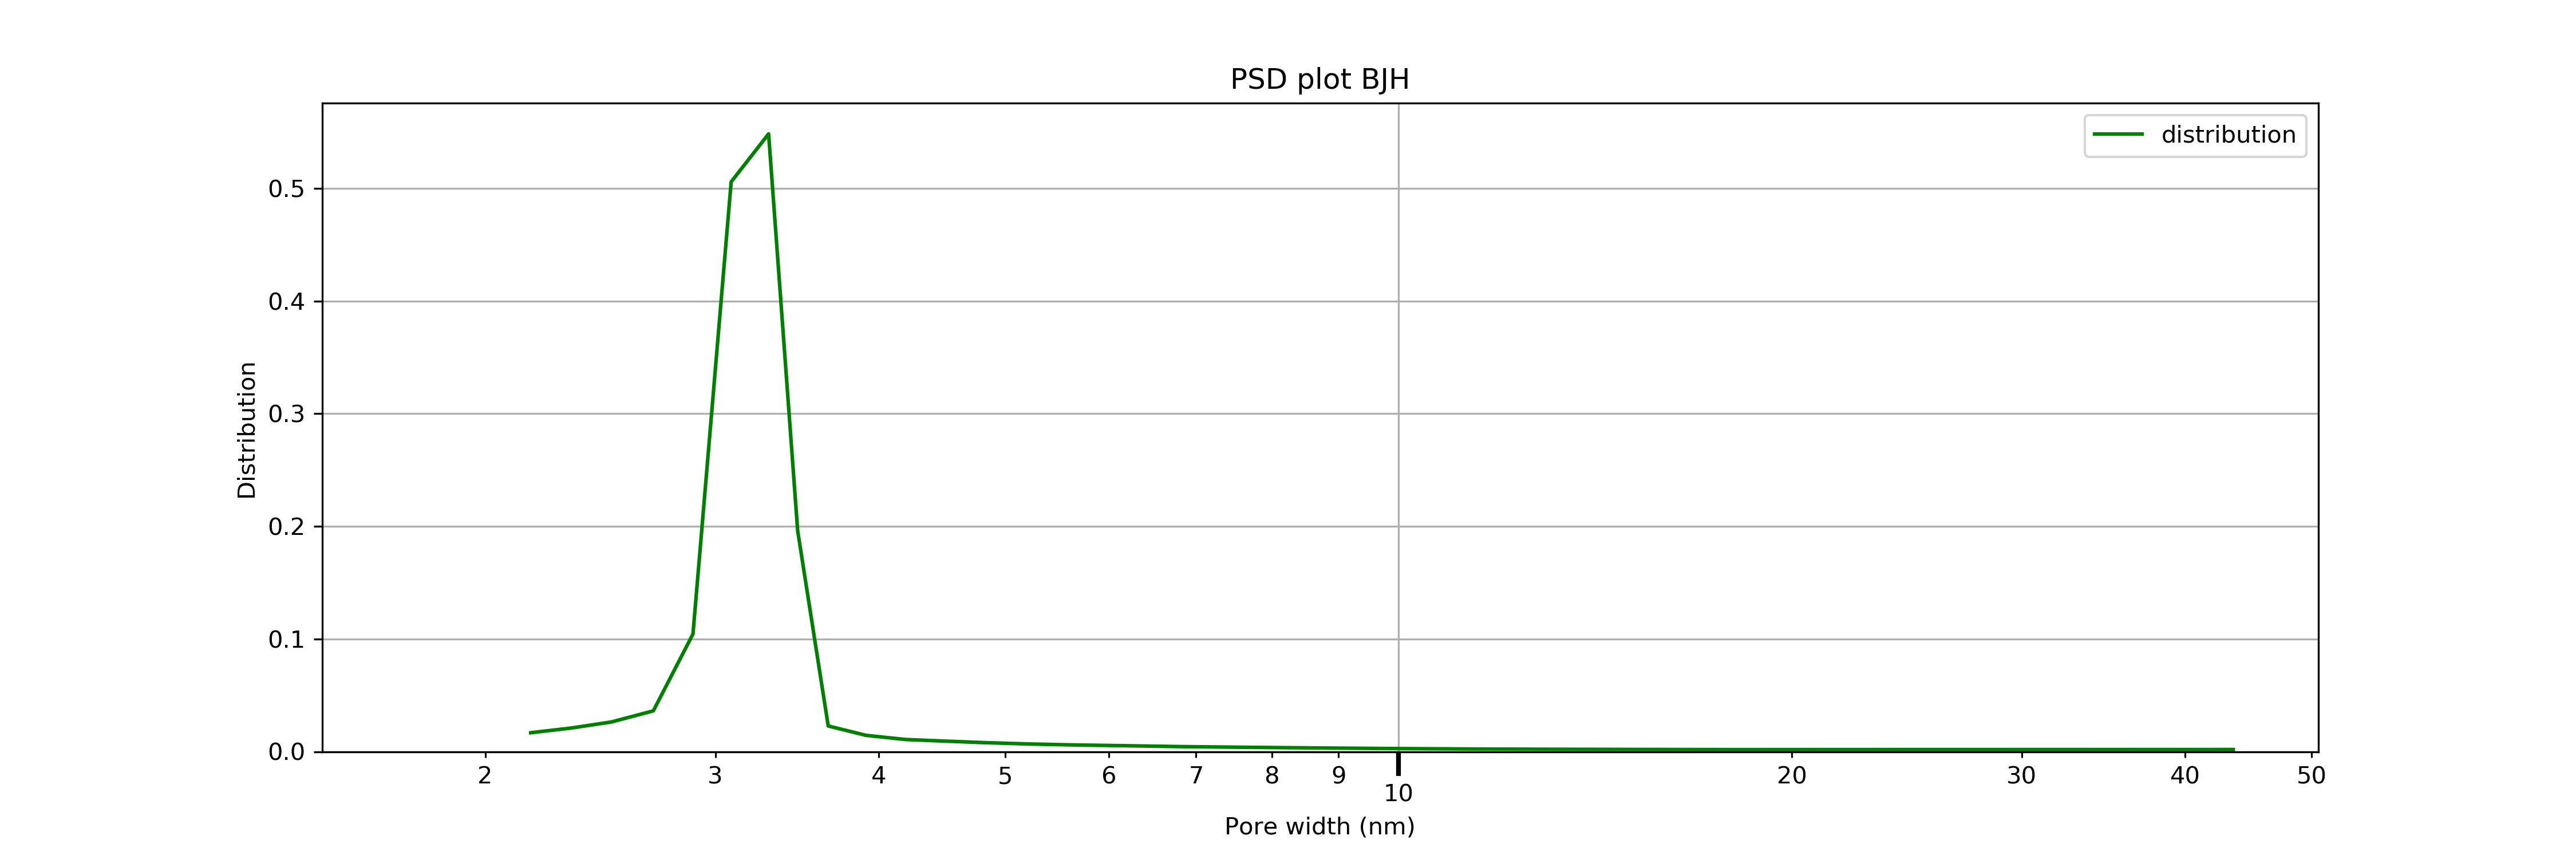
\includegraphics[width=\linewidth]{psd/bjh-des}
	\caption{BJH pore size distribution}%
	\label{pyg:fig:bjhplot}
\end{figure}

The resulting pore size distribution in \autoref{pyg:fig:bjhplot},
confirms the analysis, with a single sharp pore distribution 
at \SI{3}{\nano\metre}.

A microporous analysis cannot be performed on MCM-41, since 
it does not contain any pores under \SI{2.5}{\nano\metre}, 
where such methods are applicable. Instead, the UiO-66(Zr)
isotherm is used. This \gls{MOF} has two micropores, a tetrahedral
and an octahedral one, which are accessible through an \SI{0.8}{\nano\metre}
window. The \gls{HK} method is used for calculating the pore size 
distribution, as displayed in \autoref{pyg:lst:hkpsd}.

\begin{python}[float=htb, caption={Using the HK method for PSD},%
    label={pyg:lst:hkpsd}]
# Calling the HK micropore method with the 
# Saito-Foley oxide surface parameters
result_dict = pygaps.micropore_size_distribution(
    isotherm,
    psd_model='HK',
    adsorbent_model='OxideIon(SF)',
    verbose=True
)
# Defining a custom adsorbate parameter dictionary 
# and using it in the HK method
adsorbate_params = {
    'magnetic_susceptibility': 3.6e-35,
    'molecular_diameter': 0.3,
    'polarizability': 1.76e-30,
    'surface_density': 6.71e+18
}
result_dict = pygaps.micropore_size_distribution(
    isotherm,
    psd_model='HK',
    adsorbent_model='OxideIon(SF)',
    adsorbate_model=adsorbate_params,
    verbose=True
)
\end{python}

\begin{figure}[!htb]
	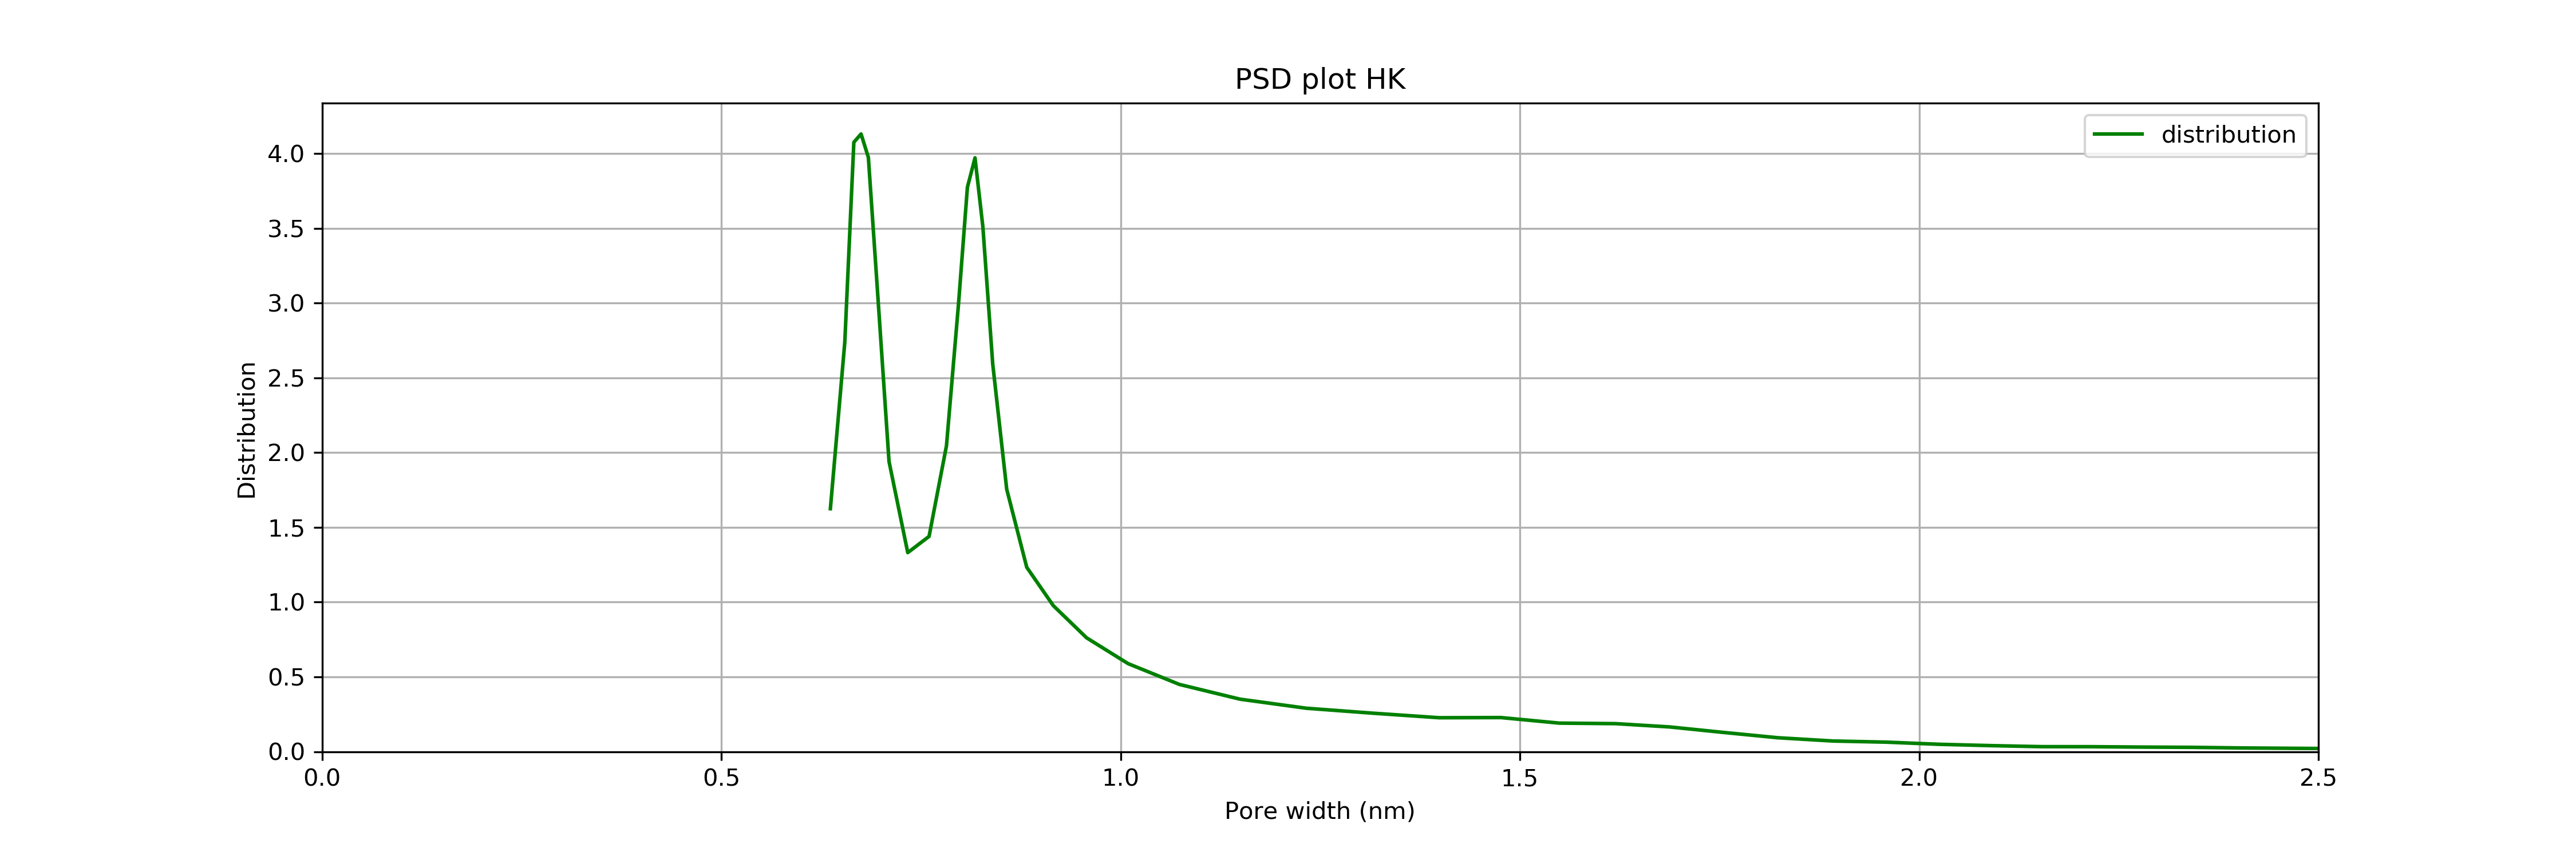
\includegraphics[width=\textwidth]{psd/hk}
	\caption{Pore size distribution calculated through the Horvath-Kawazoe method on the UIO-66(Zr) sample}%
	\label{fig:pyg:fig:hk}
\end{figure}

The \texttt{pyGAPS} framework contains the required physical properties
for the most commonly used adsorbates in its database, as well as
properties from literature for several materials:
the original parameters developed by Horvath and Kawazoe for a 
carbon surface~\cite{horvathMethodCalculationEffective1983} and the
oxide surface parameters published by Saito and
Foley~\cite{saitoCurvatureParametricSensitivity1991}.
The user can also provide a custom dictionary for these parameters
when calling the function as can be seen in the second example
in \autoref{pyg:lst:hkpsd}.

Finally, to determine a pore size distribution using \gls{DFT} kernel fitting,
the \inline{dft_size_distribution} function is used. 
The function takes an \texttt{Isotherm} object and a path
to a CSV representation of the \gls{DFT} kernel. The code then
loads the kernel either from disk or memory and 
applies a minimization function on the sum of squared differences
of the sum of all individual kernel isotherms to generate 
the contribution of each as per the following equation:

\begin{equation}
	f(x) = \sum_{p=p_0}^{p=p_x} \Big(n_{p,exp} - \sum_{w=w_0}^{w=w_y} n_{p, kernel} X_w \Big)^2
\end{equation}

The user can specify their own kernel in a CSV format or, alternatively,
use the internal kernel is included with the framework. This kernel
is only applicable on \ce{N2} adsorption at \SI{77}{\kelvin} on 
carbon slit-like pores in the range of \SIrange{0.4}{10}{\nano\meter}.

The isotherm measured on the microporous carbon Takeda 5A is used as 
an input for the \gls{DFT} fitting routine (\autoref{pyg:lst:dft}), using the
available internal kernel. The resulting PSD shows that the material
is not completely microporous, with a wide mesopore component
present.

\begin{python}[caption={DFT size distribution in pyGAPS},%
    label={pyg:lst:dft}]
result_dict = pygaps.dft_size_distribution(
    charact_iso,
    'internal',
    verbose=True
)
\end{python}
\begin{figure}[!htb]
	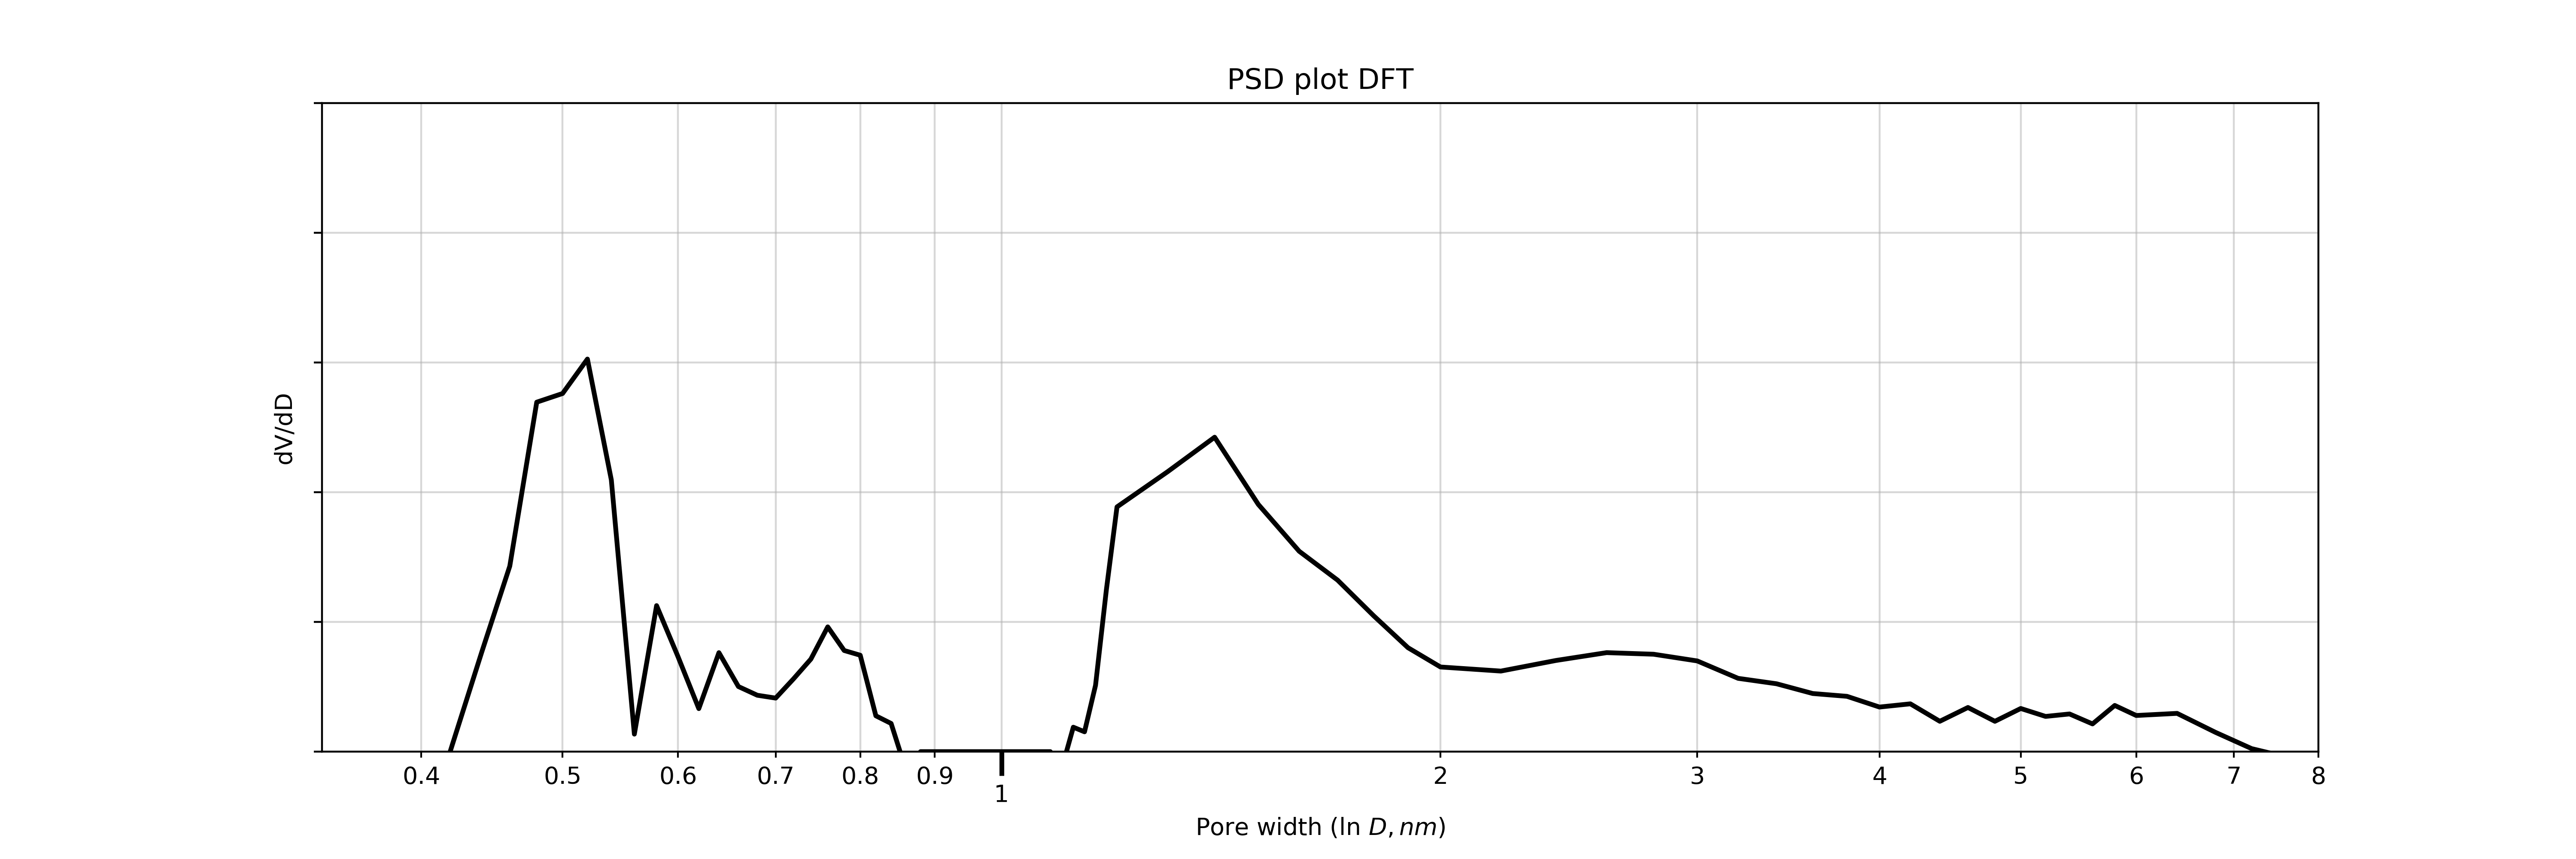
\includegraphics[width=\textwidth]{psd/dft-plt}
	\caption{Pore size distribution calculated through the \gls{DFT} fitting on the Takeda 5A carbon}%
	\label{fig:pyg:fig:dft}
\end{figure}

\subsubsection{Multicomponent adsorption modelling}

The \texttt{pyGAPS} framework includes a modified version of 
the pyIAST code~\cite{simonPyIASTIdealAdsorbed2016} which has 
been adapted to work with the \texttt{Isotherm} 
classes. Both model isotherms and real data can be used for 
\gls{IAST}, with spreading pressure being calculated through the 
underlying isotherm model or through interpolation, respectively
as detailed in \autoref{pyg:iast}.

As an example, two common case studies will be examined: the capture of
\ce{CO2} from \ce{N2} and separation of propane and propylene.
Models of isotherms recorded on a Takeda 5A microporous carbon are
generated using the automatic fitting functionality. 
The original isotherms and the best-fitting models are displayed in 
\autoref{pyg:fig:takedaco2n2iso} for the \ce{CO2}-\ce{N2} pair and 
in \autoref{pyg:fig:takedac3h6c3h8iso} for the \ce{C3H8}-\ce{C3H6} pair.

For the carbon dioxide separation, all equilibrium
points for the adsorbed and gaseous phases are simulated 
at different proportions of the two gases, with a total pressure
of \SI{1}{\bar}. To do this we use the \inline{pygaps.iast_vle()}
function which produces an analogue of a vapour-liquid equilibrium at 
a specified pressure for a binary mixture. The resulting graph can be seen
in \autoref{pyg:fig:takedac3h6c3h8iast}.
As expected, the predicted adsorbed mixture is rich in carbon dioxide.
Selectivity can also be calculated in a single point, with the value at
a concentration analogous to flue gas of 15\% \ce{CO2} being 16.5. 

\begin{figure}[htb]

    \centering
    \begin{subfigure}[b]{.42\textwidth}
        \centering
        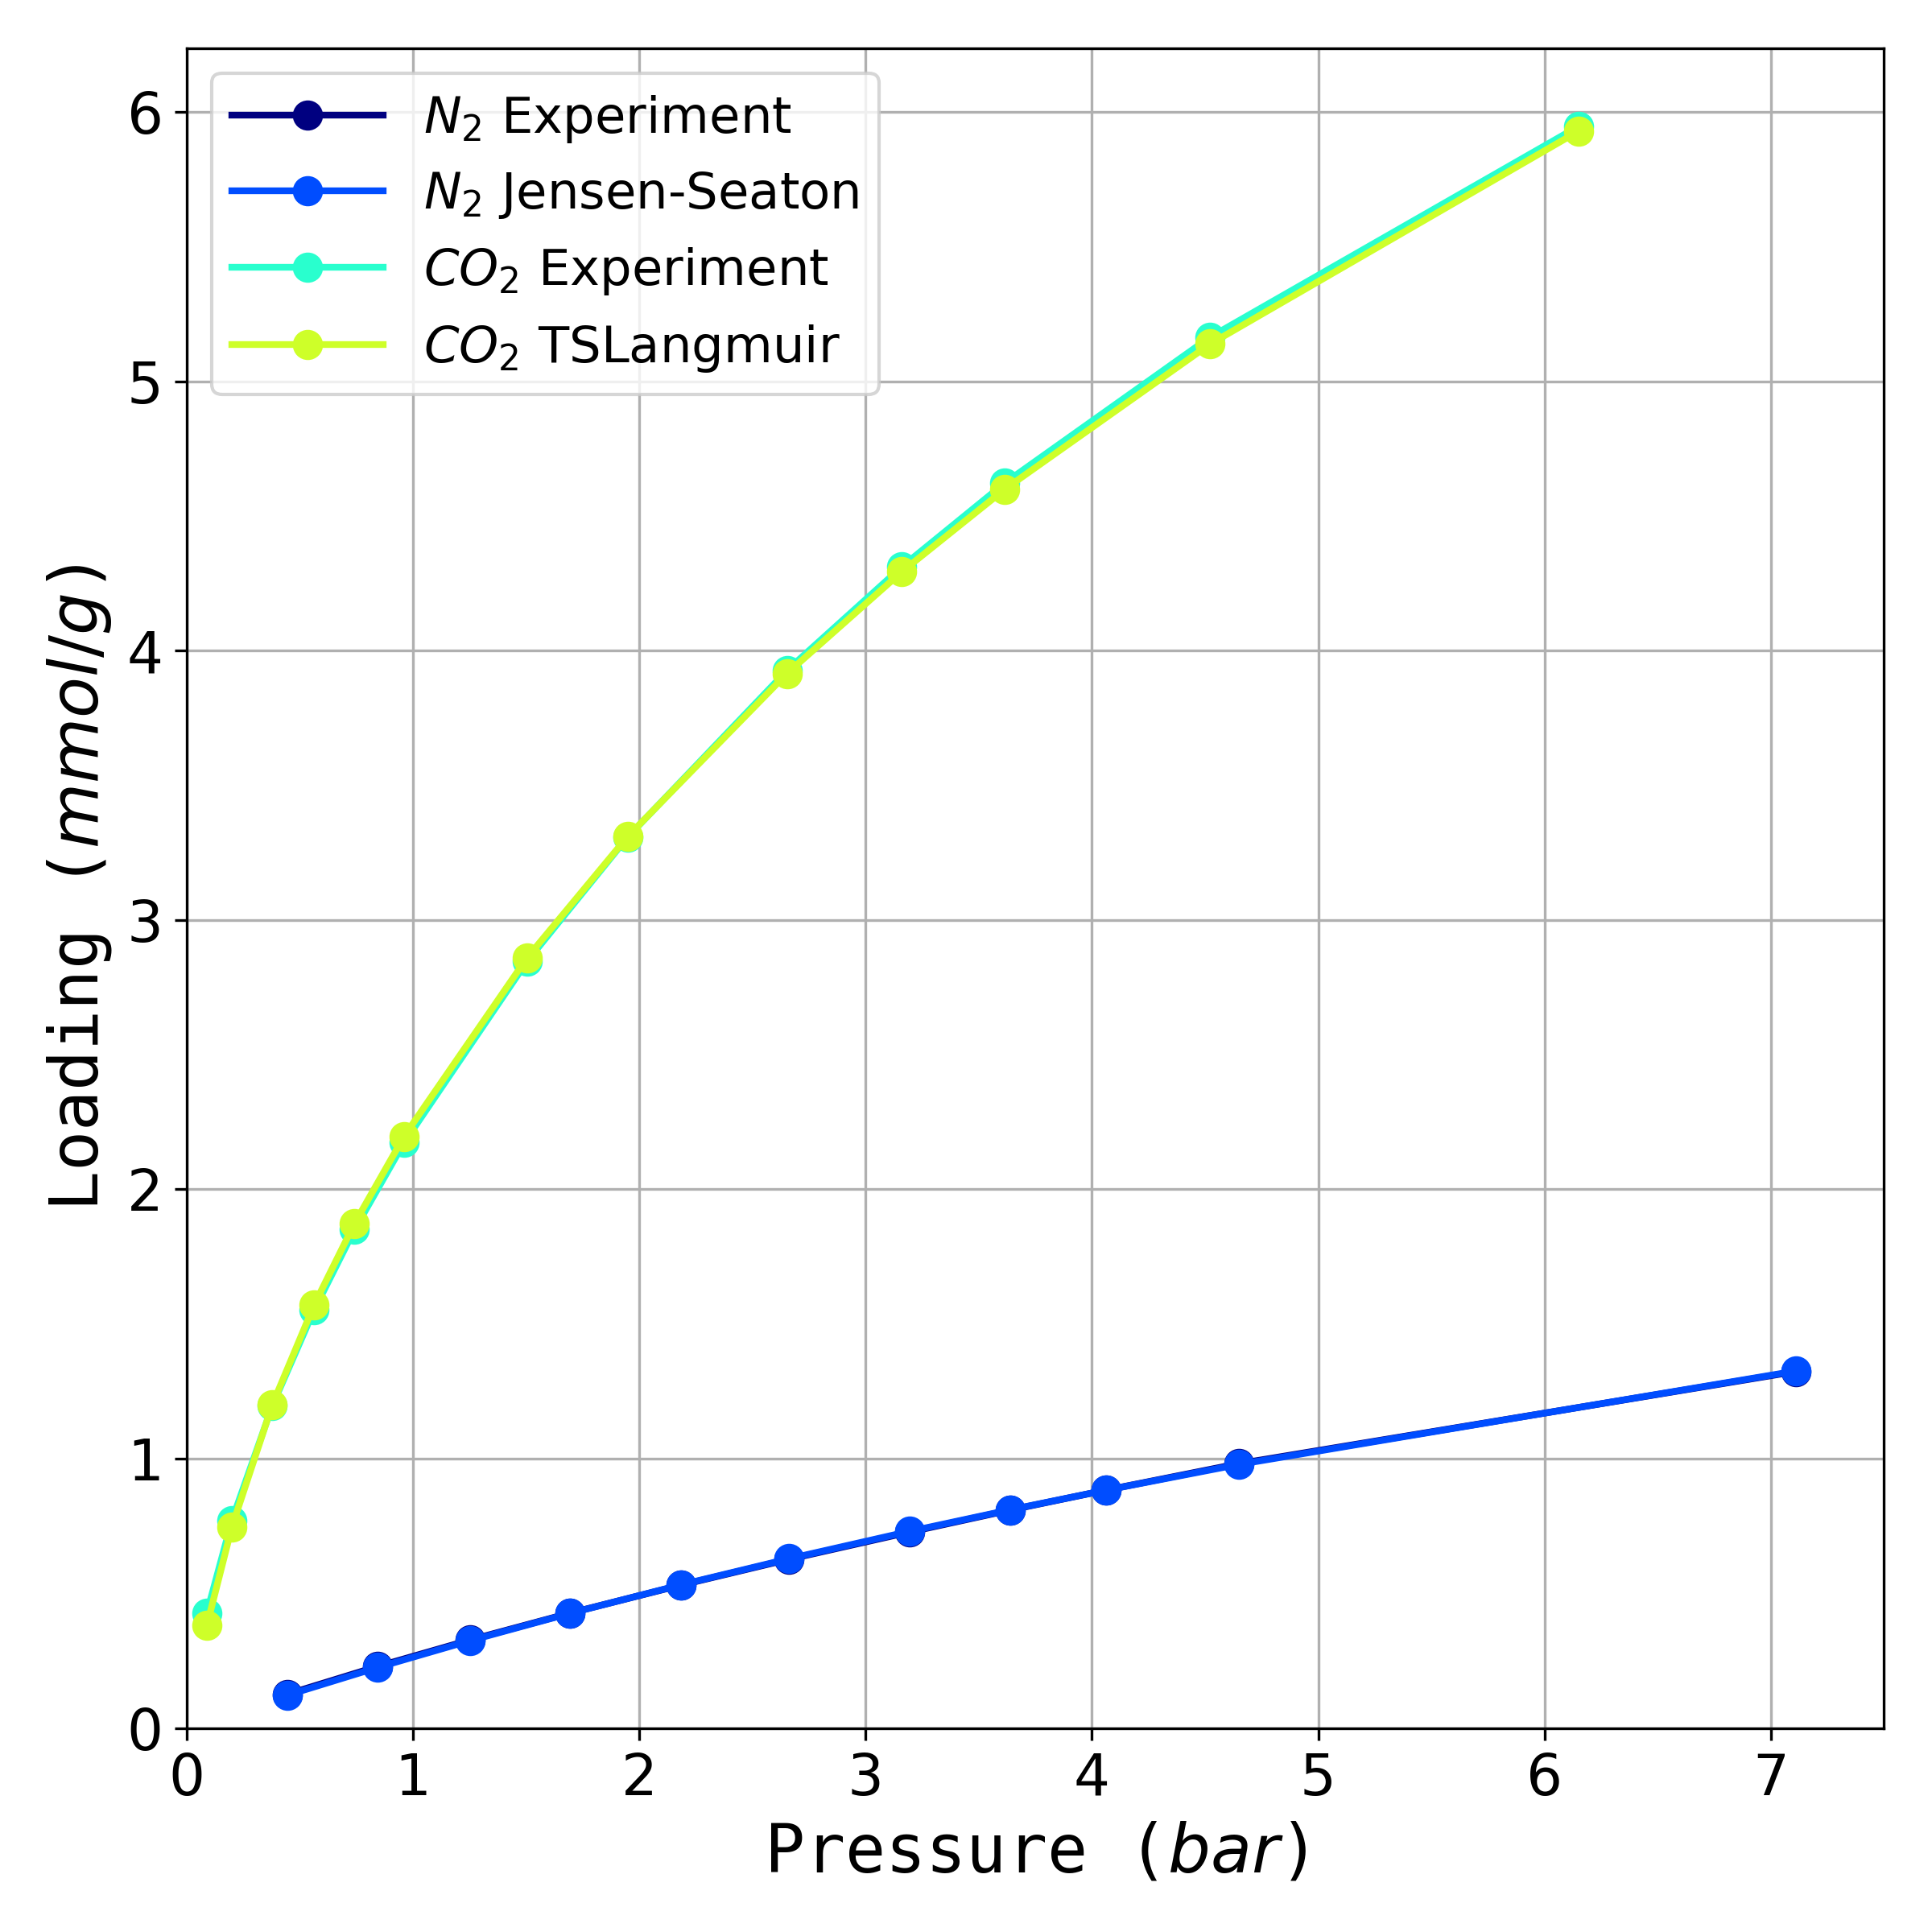
\includegraphics[width=.8\linewidth]{iast/takeda-co2n2}
        \caption{}%
        \label{pyg:fig:takedaco2n2iso}
    \end{subfigure}%
    \begin{subfigure}[b]{.4\textwidth}
        \centering
        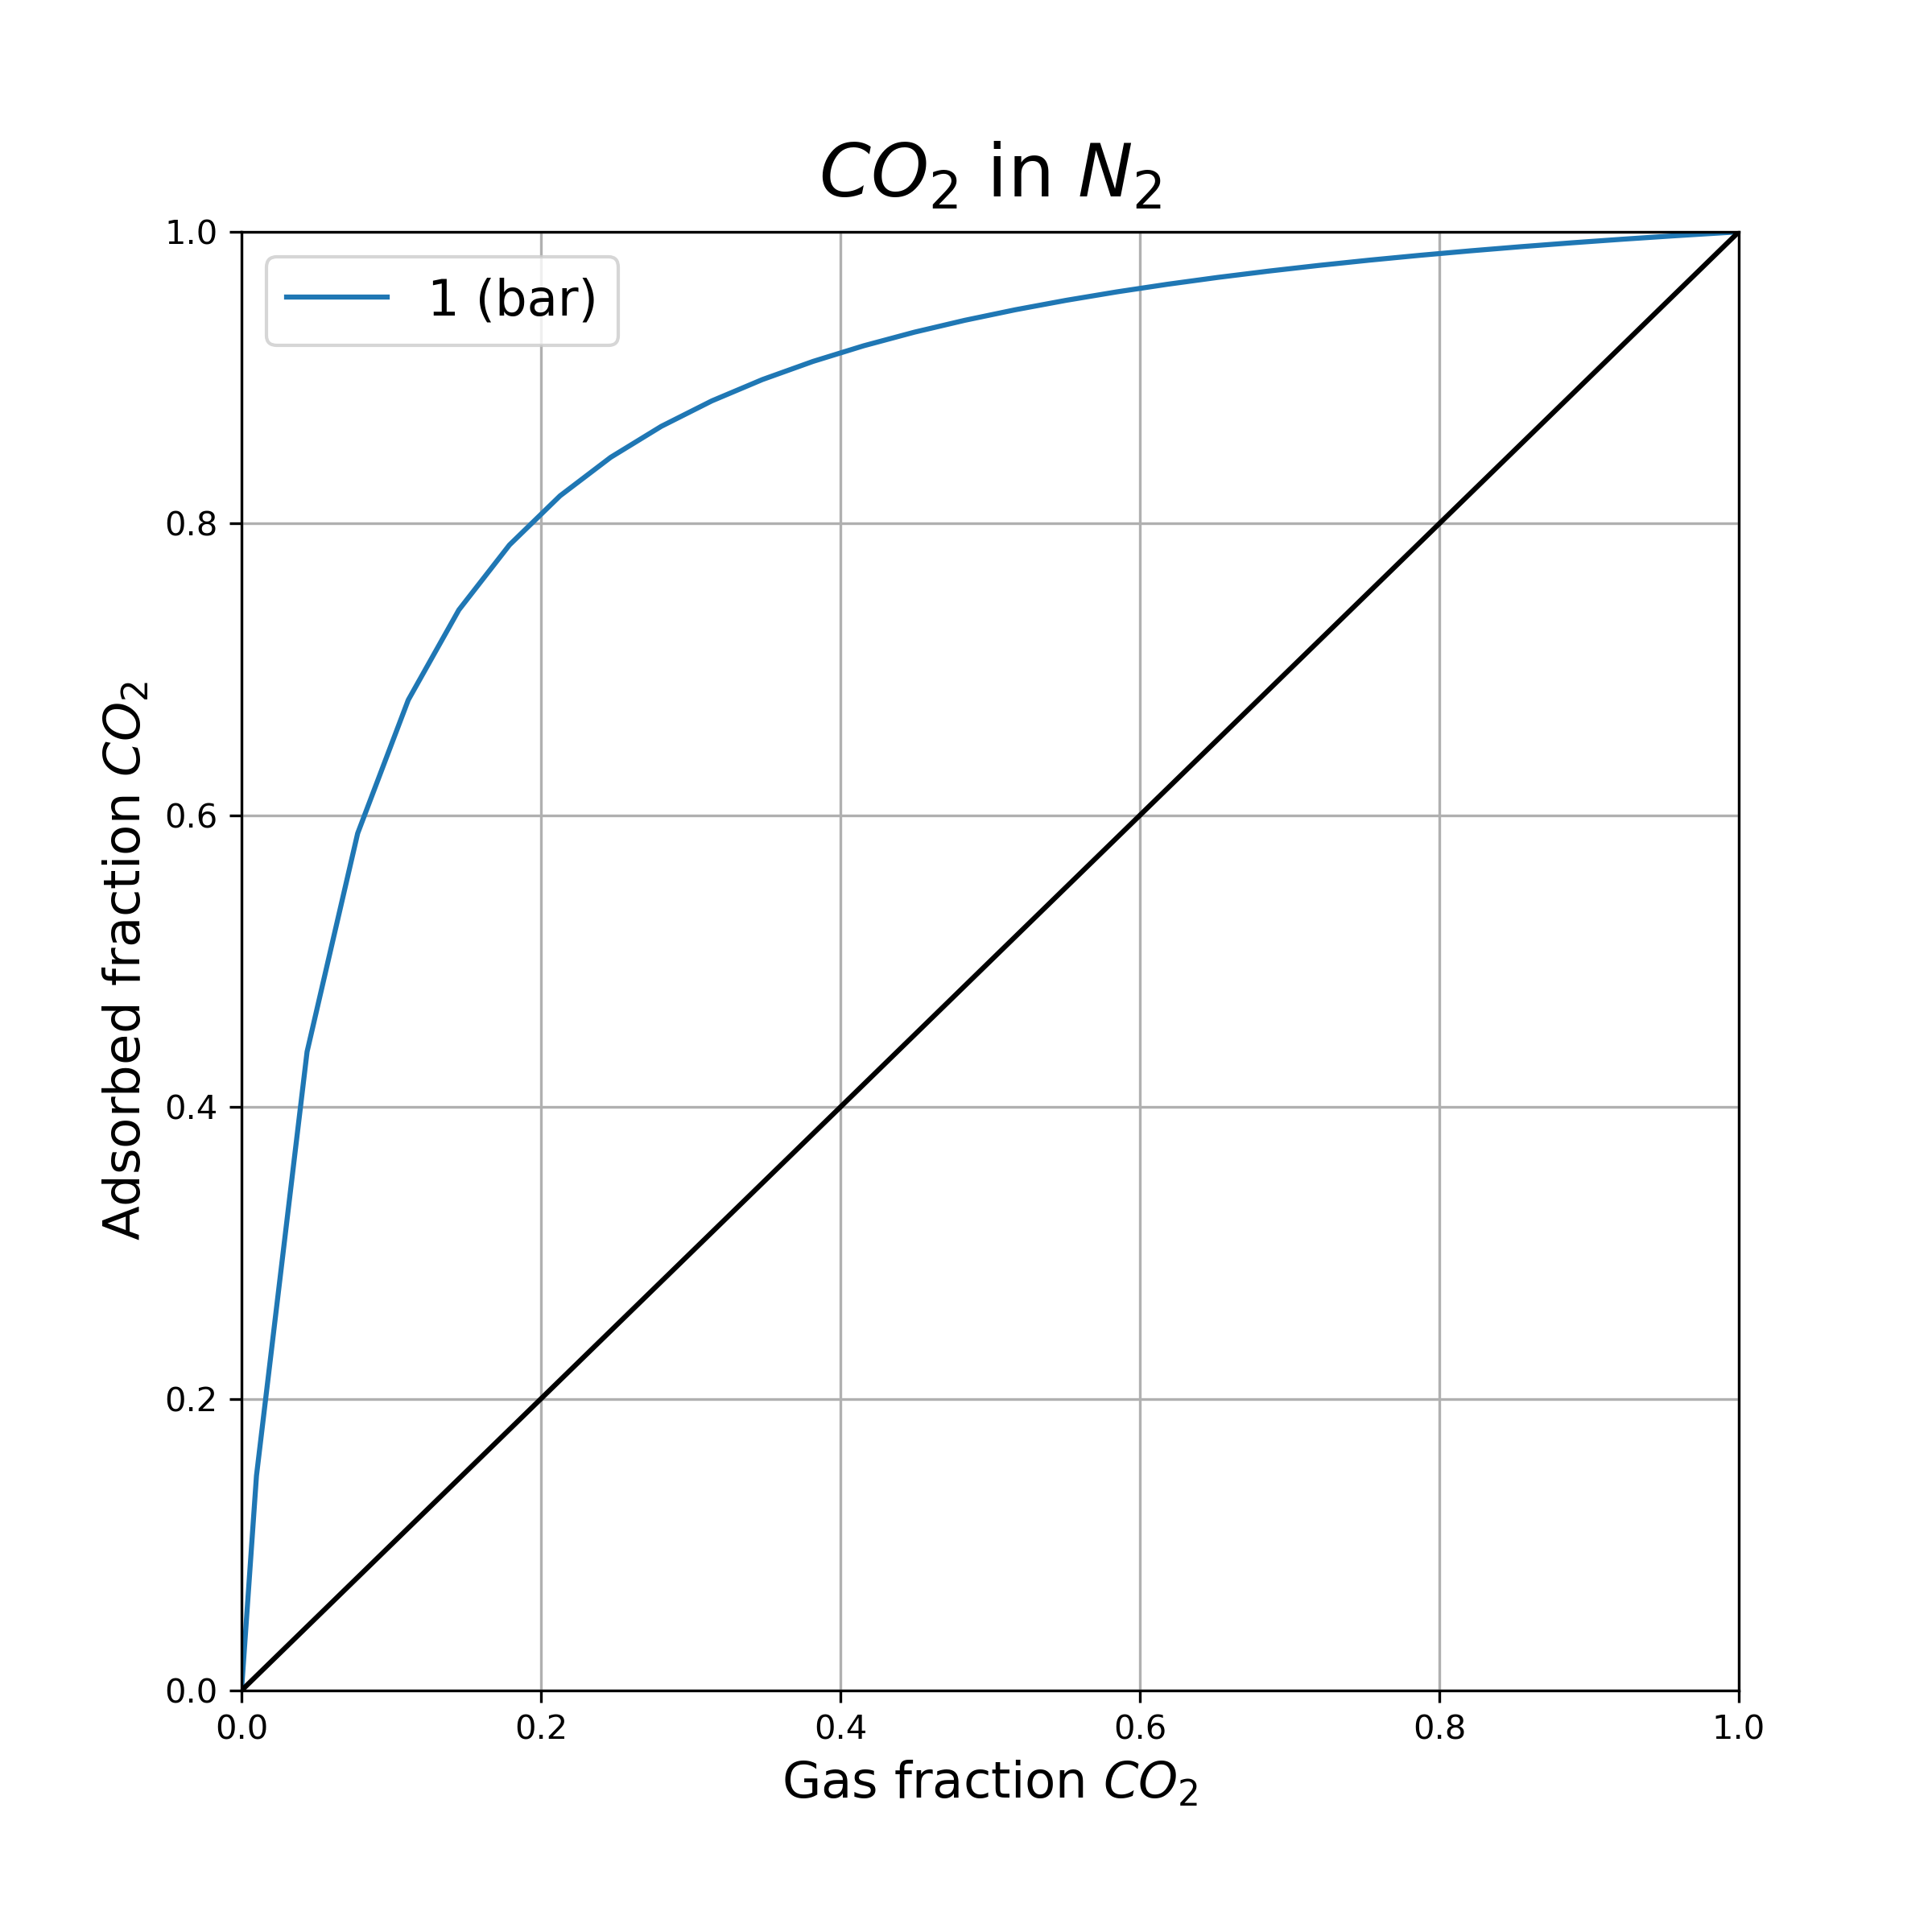
\includegraphics[width=0.92\linewidth]{iast/takeda-co2n2-vle}
        \caption{}%
        \label{pyg:fig:takedaco2n2iast}
    \end{subfigure}
    \caption{
    Modelling binary adsorption of \ce{CO2} and \ce{N2}: 
    (\protect\subref{pyg:fig:takedaco2n2iso}) the pure component
    isotherms and their best fit models and 
    (\protect\subref{pyg:fig:takedaco2n2iast}) 
    the predicted composition of the gaseous
    and adsorbed phase for different fractions of 
    \ce{CO2} at \SI{1}{\bar}
    }%
    \label{pyg:fig:takedaco2n2}

\end{figure}

For the propane-propylene separation, the selectivity for
propane in an equimolar mixture of the two gases is simulated within
a pressure range of \SIrange{0.1}{5}{\bar}. 
It can be seen that there is little or no preference for the 
unsaturated molecule, though the selectivity increases slightly at 
pressures above \SI{1}{\bar}.

\begin{figure}[htb]

    \centering
    \begin{subfigure}[b]{.42\textwidth}
        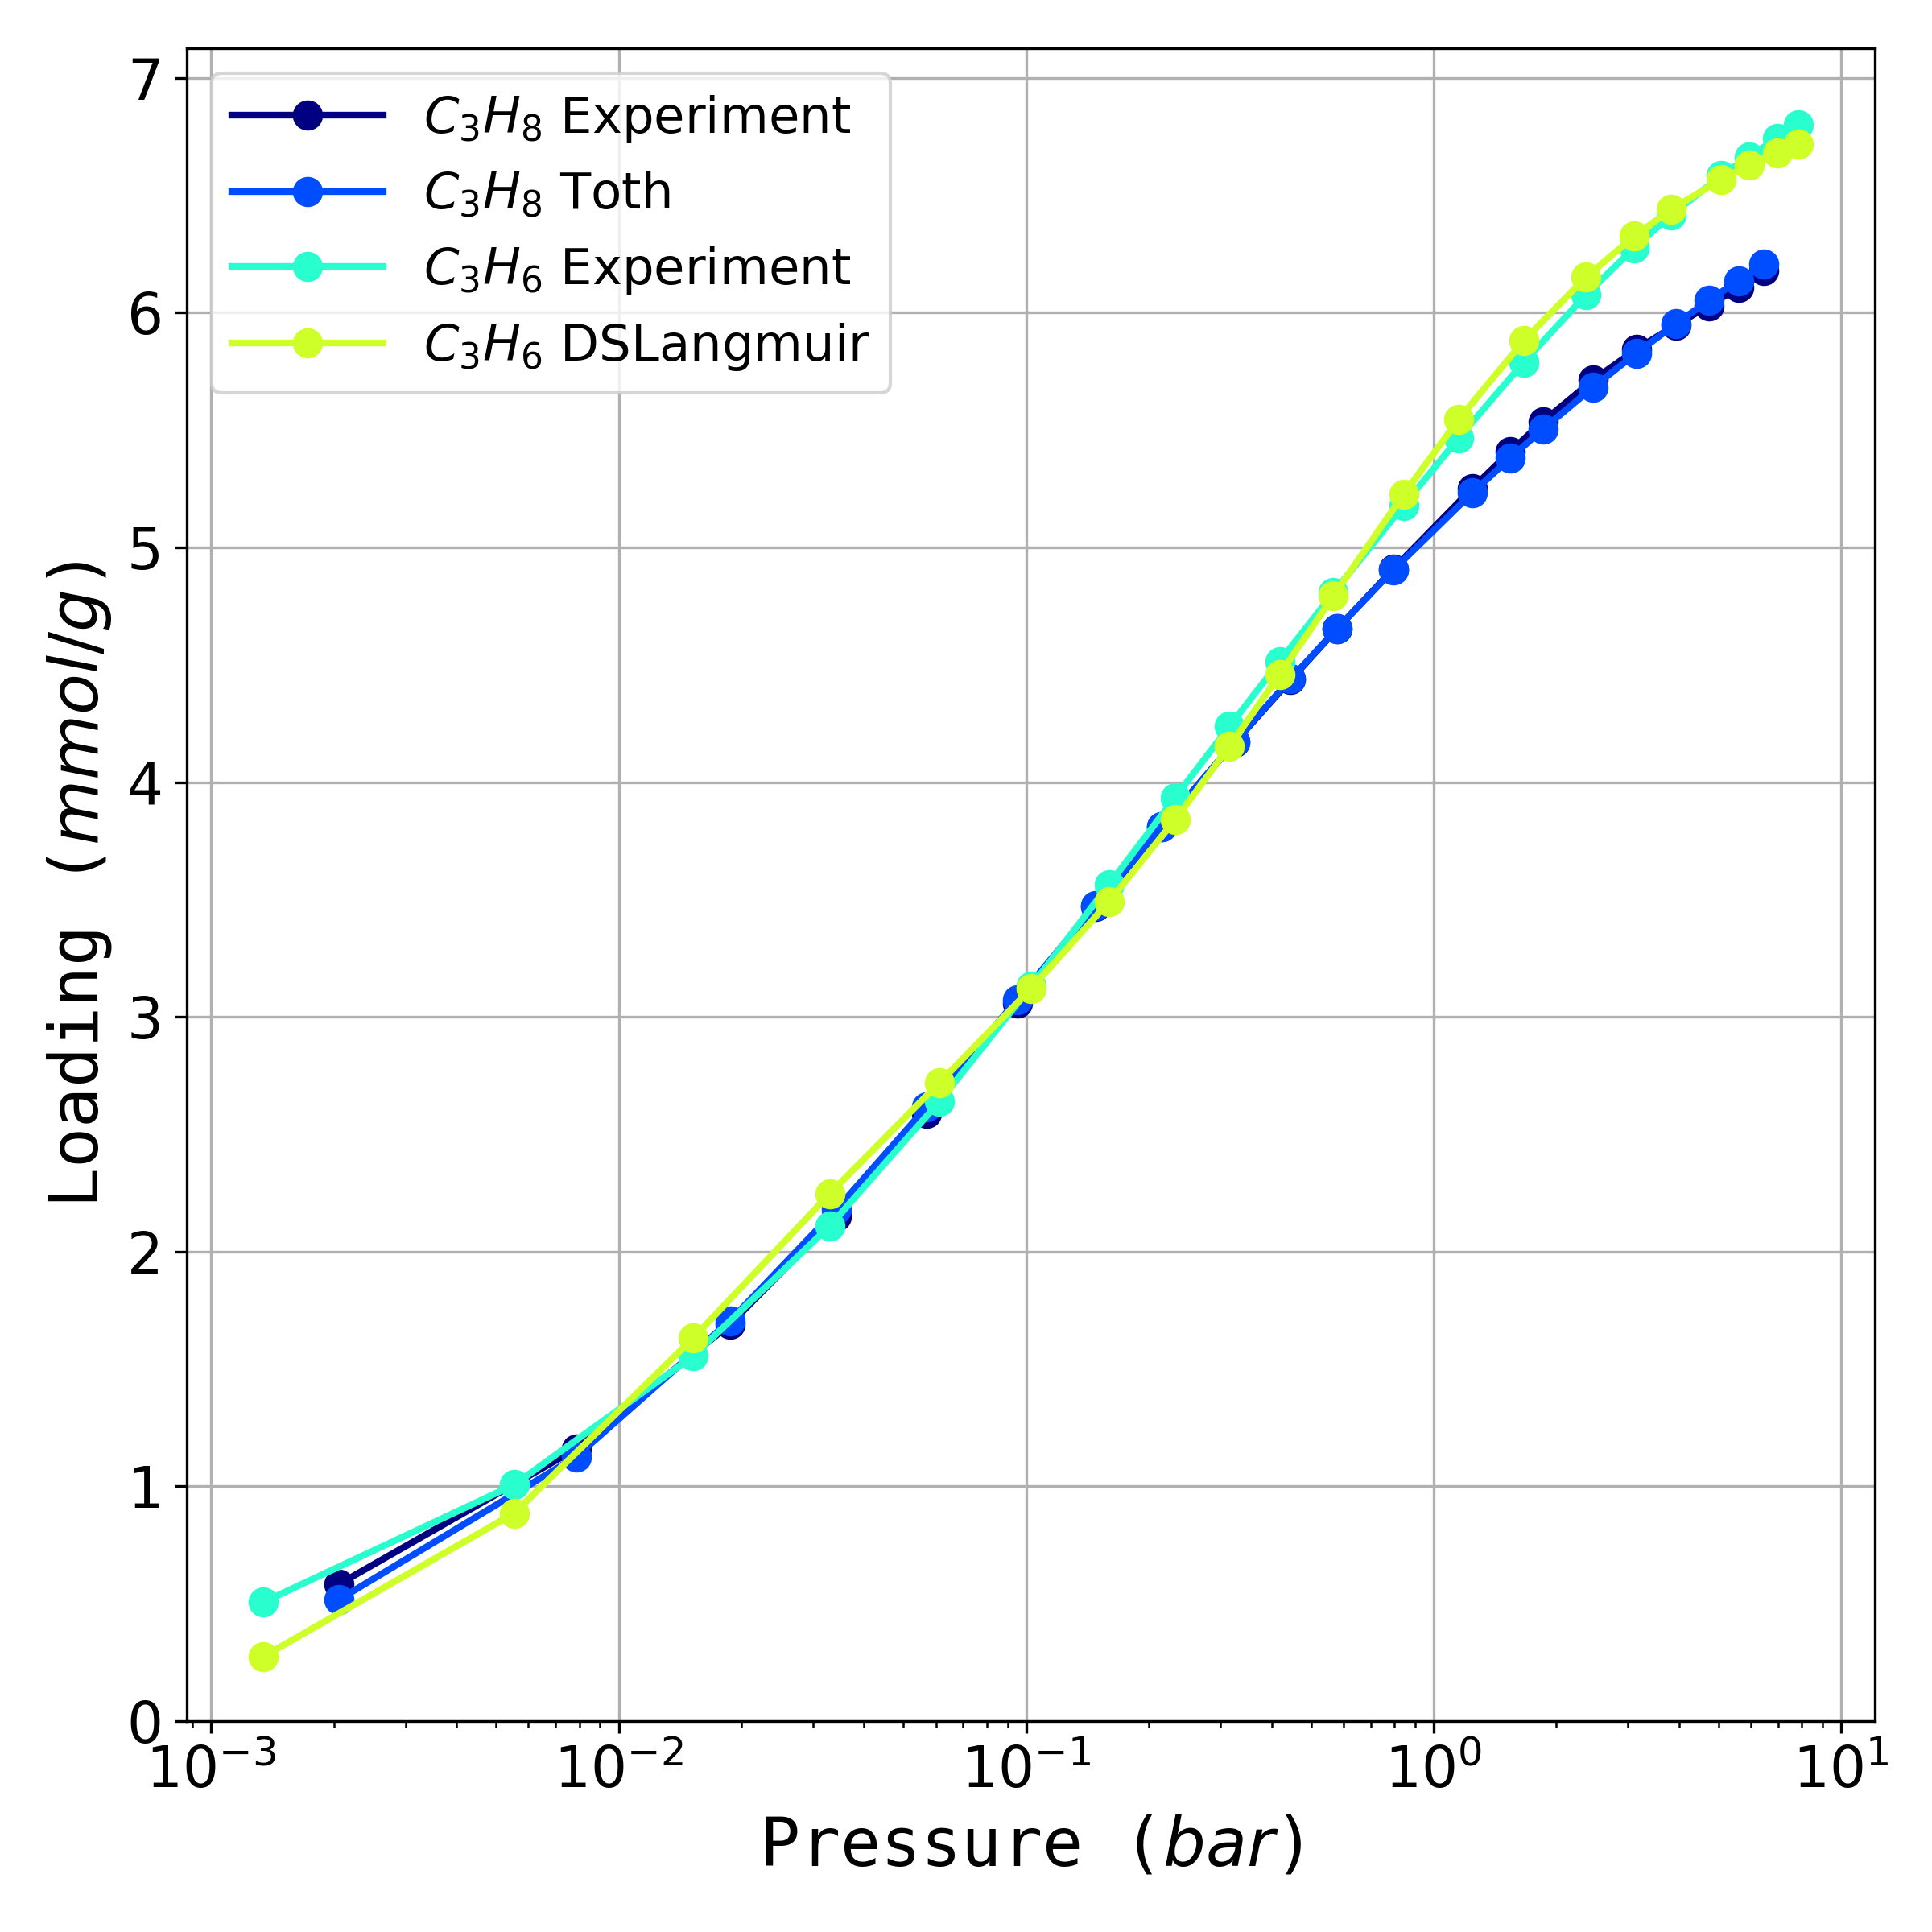
\includegraphics[width=.9\linewidth]{iast/takeda-c3h6c3h8}
        \caption{}%
        \label{pyg:fig:takedac3h6c3h8iso}
    \end{subfigure}
    \begin{subfigure}[b]{.4\textwidth}
        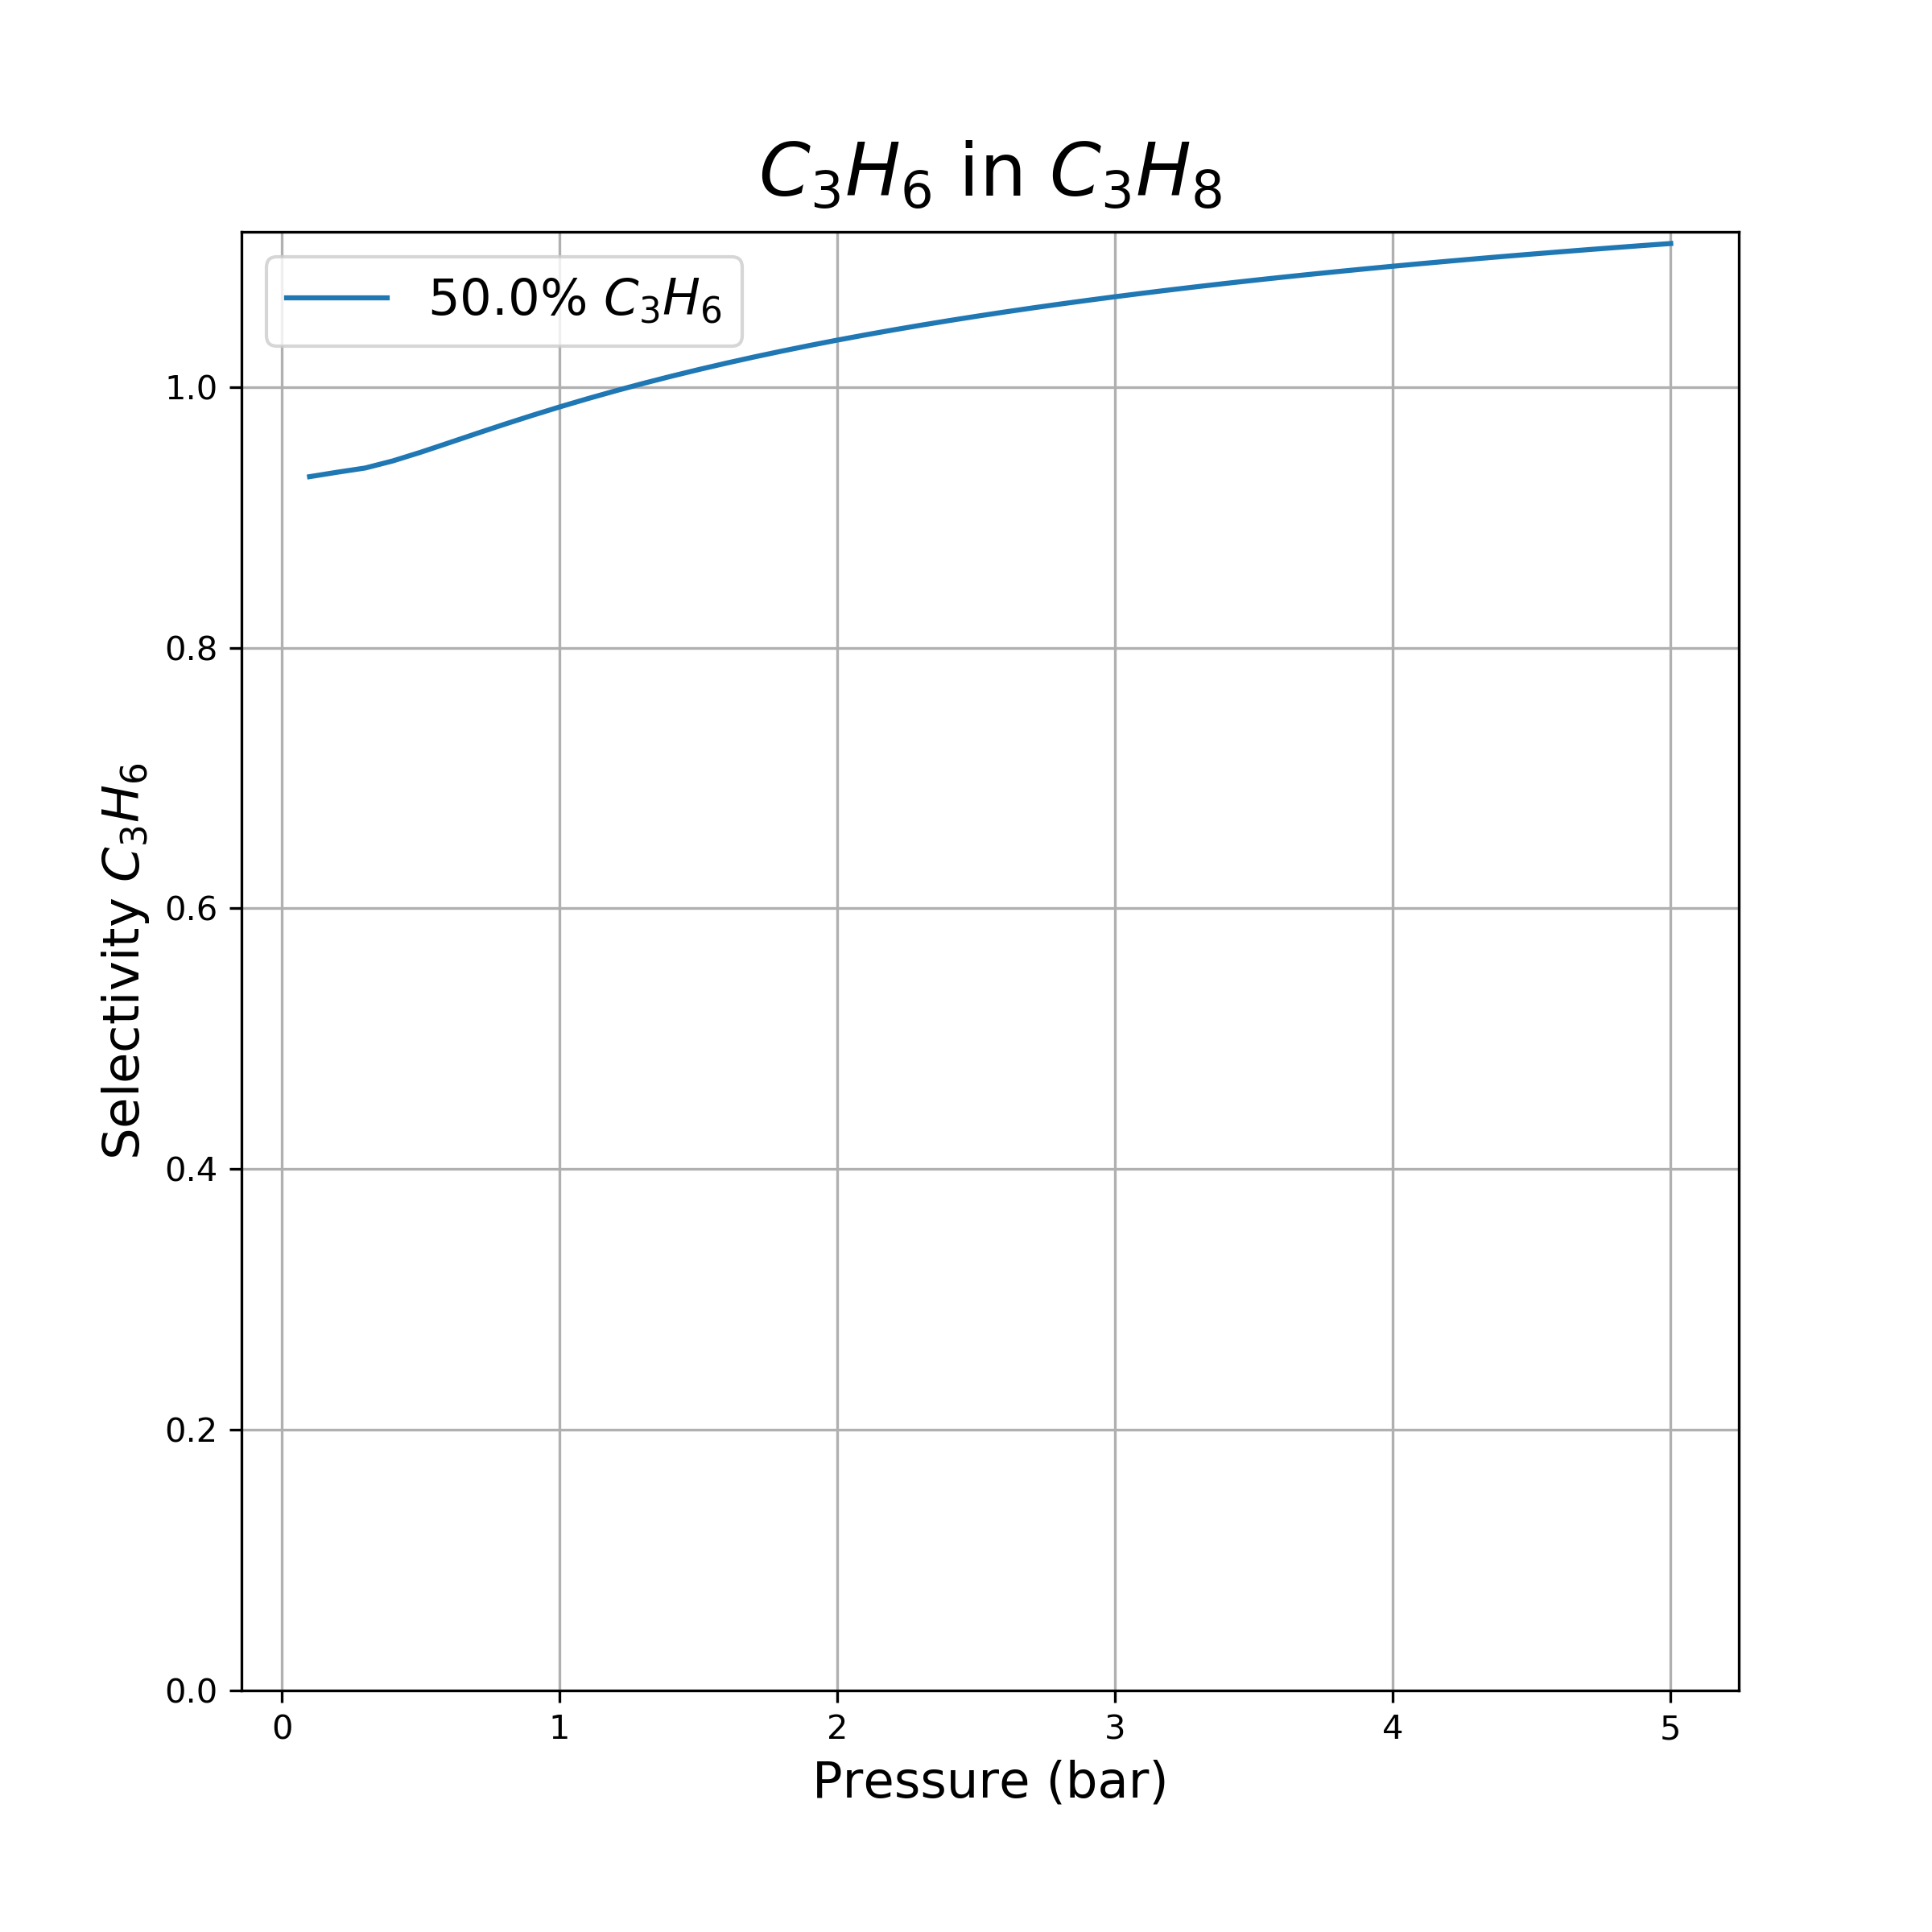
\includegraphics[width=\linewidth]{iast/takeda-c3h6c3h8-svp}
        \caption{}%
        \label{pyg:fig:takedac3h6c3h8iast}
    \end{subfigure}
    \caption{%
    Modelling binary adsorption of a propane-propylene mixture: 
    (\protect\subref{pyg:fig:takedac3h6c3h8iso}) the pure-component
    isotherms and their best fit models and 
    (\protect\subref{pyg:fig:takedac3h6c3h8iast})
    the predicted selectivity of propane adsorption 
    of a 50--50\% mixture in a range of pressure from 0.1 to 7 bar}%
    \label{pyg:fig:takedac3h6c3h8}

\end{figure}